\documentclass{article}
\usepackage[margin=1in]{geometry}
\usepackage{graphicx}
\usepackage{booktabs}
\usepackage{float}
\usepackage{amsmath}
\usepackage{amssymb}
\usepackage{threeparttable}
\usepackage{longtable}
\graphicspath{{./}{overleaf_images/}}

\title{Project 2}
\author{Disha Dhangar, Adithya Lakshmikanth, Aastha Mishra, Ellie Truong, Amy Vu}
\date{October 2026}

\begin{document}

\maketitle

\section{Introduction}

This report presents a regression and symbolic regression analysis across three benchmark datasets. The analysis includes multiple regression, regularized regression using Ridge and Lasso, forward feature selection, transformed regression, and symbolic regression. ScalaTion (Scala 3) is used across all five modeling approaches, while Python's \texttt{statsmodels} is used for multiple and regularized regression and \texttt{PySR} is used for symbolic regression. Across the required cases, model results and evaluation measures are presented and discussed to examine model fit, predictive performance, and the effects of different regression techniques.



The cleaned UCI data contain 392 rows and 8 numeric columns for Auto MPG (target MPG), 1,030 rows and 9 columns for Concrete (target compressive strength in MPa), and 1,503 rows and 6 columns for Airfoil (target scaled sound pressure in dB). Auto MPG's 398-row numeric source has six missing-horsepower rows; removing those rows and excluding car names yields the 392-row modeling file. Direct comparison with the supplied UCI archives confirms the cleaned values and row order (Concrete differs only at floating-point roundoff). The report covers 12 ScalaTion cases, 5 \texttt{statsmodels} cases, and 3 PySR cases: 20 total. Log, square root, and Box--Cox are applied to the response for each of the two transformed-regression datasets.

\section{Multiple Regression}

Multiple regression is used to predict a single outcome from multiple independent variables while estimating the association between each predictor and the response conditional on the other predictors. For each dataset, a multiple regression model was fitted using all available predictors in both ScalaTion and \texttt{statsmodels}, giving six required regression models. Additional simple regression models were fitted using the two predictors with the largest absolute correlations with the response variable. The same predictor selections were used for the ScalaTion and \texttt{statsmodels} analyses. All $R^2$ values reported for the full regression models are in-sample values computed using the full datasets and are therefore not directly comparable to held-out test-set metrics reported in later sections.

\subsection{ScalaTion}

The ScalaTion implementation used an intercept term and all available predictors for each of the multiple regression models. The fitted models were evaluated using the reported $R^2$, adjusted $R^2$, residual standard error, and fitted coefficient statistics. Simple regression models were also fitted for the two predictors with the largest absolute correlations with each response variable.

\subsubsection{Auto MPG}

For the Auto MPG dataset, the full multiple regression model uses cylinders, displacement, horsepower, weight, acceleration, model year, and origin to predict MPG. The resulting model showed a strong overall fit, with an $R^2$ of approximately 0.821. Substantial multicollinearity was present among several vehicle characteristics. The VIF values from ScalaTion were above 10 for cylinders, displacement, and weight, with displacement having the highest VIF at approximately 21.84. The two predictors with the largest absolute correlations with MPG were weight and displacement. Both simple regression models showed a negative relationship with MPG, with higher vehicle weight and displacement corresponding to lower predicted MPG.

\begin{table}[H]
\centering
\small
\caption{Auto MPG full regression coefficients from ScalaTion.}
\label{tab:auto-scalation-coefficients}
\begin{tabular}{lrrrrr}
\hline
Predictor & Estimate & Std. Error & t & $p$ & VIF \\
\hline
Intercept    & -17.2184 & 4.6443  & -3.71  & 0.0002   & -- \\
Cylinders    & -0.4934  & 0.3233  & -1.53  & 0.1270   & 10.74 \\
Displacement & 0.01990  & 0.00752 & 2.65   & 0.0081   & 21.84 \\
Horsepower   & -0.01695 & 0.01379 & -1.23  & 0.2189   & 9.94 \\
Weight       & -0.00647 & 0.00065 & -9.93  & $<$0.001 & 10.83 \\
Acceleration & 0.0806   & 0.0988  & 0.82   & 0.4150   & 2.63 \\
Model year   & 0.7508   & 0.0510  & 14.73  & $<$0.001 & 1.24 \\
Origin       & 1.4261   & 0.2781  & 5.13   & $<$0.001 & 1.77 \\
\hline
\end{tabular}
\end{table}

For Auto MPG, weight, model year, and origin were statistically significant predictors in the full model at $p<0.001$. Weight had a negative coefficient, while model year and origin had positive coefficients. Displacement also had a positive coefficient and was significant at $p=0.008$, despite its negative simple-regression relationship with MPG. This difference illustrates the effect of controlling for correlated predictors in a multiple regression model. The high VIF values for displacement, cylinders, and weight indicate substantial multicollinearity, so individual coefficient estimates should be interpreted with caution.





\subsubsection{Concrete}

For the Concrete dataset, the full multiple regression model used cement, blast furnace slag, fly ash, water, superplasticizer, coarse aggregate, fine aggregate, and age to predict compressive strength. The resulting model showed an $R^2$ of approximately 0.615. The two predictors with the largest absolute correlations with compressive strength were cement and superplasticizer, and both showed positive simple regression relationships with compressive strength. The Concrete predictors also showed some multicollinearity. Several VIF values were above 5, including cement, blast furnace slag, fly ash, water, coarse aggregate, and fine aggregate. These elevated VIF values indicate that several predictors are correlated with the other predictors in the model, which can make individual coefficient estimates more difficult to interpret.

\begin{table}[H]
\centering
\small
\caption{Concrete full regression coefficients from ScalaTion.}
\label{tab:concrete-scalation-coefficients}
\begin{tabular}{lrrrrr}
\hline
Predictor & Estimate & Std. Error & t & $p$ & VIF \\
\hline
Intercept           & -23.1638 & 26.5884 & -0.87 & 0.3836   & -- \\
Cement              & 0.1198   & 0.0085  & 14.11 & $<$0.001 & 7.49 \\
Blast furnace slag  & 0.1038   & 0.0101  & 10.25 & $<$0.001 & 7.28 \\
Fly ash             & 0.0879   & 0.0126  & 6.99  & $<$0.001 & 6.17 \\
Water               & -0.1503  & 0.0402  & -3.74 & 0.0002   & 7.00 \\
Superplasticizer    & 0.2907   & 0.0935  & 3.11  & 0.0019   & 2.97 \\
Coarse aggregate    & 0.0180   & 0.0094  & 1.92  & 0.0549   & 5.08 \\
Fine aggregate      & 0.0202   & 0.0107  & 1.88  & 0.0597   & 7.01 \\
Age                 & 0.1142   & 0.0054  & 21.05 & $<$0.001 & 1.12 \\
\hline
\end{tabular}
\end{table}

For Concrete, cement, blast furnace slag, fly ash, water, superplasticizer, and age were statistically significant predictors at the 0.05 level. Water had a negative coefficient, while the other significant predictors had positive coefficients. Coarse aggregate and fine aggregate were not significant at the 0.05 level, with p-values of approximately 0.055 and 0.060, respectively. The elevated VIF values for several material variables indicate substantial correlation among some of the predictors.





\subsubsection{Airfoil}

For the Airfoil dataset, the full multiple regression model used frequency, angle of attack, chord length, free-stream velocity, and suction displacement thickness to predict scaled sound pressure. The full model produced an $R^2$ of approximately 0.516. The two predictors with the largest absolute correlations with scaled sound pressure were frequency and suction displacement thickness. Both simple regression models showed a negative relationship with the response. Compared with the other two datasets, the Airfoil predictors showed lower multicollinearity, with all VIF values below 3.5. Angle of attack had the highest VIF at approximately 3.44, while the remaining predictors had VIF values below 2.6.

\begin{table}[H]
\centering
\small
\caption{Airfoil full regression coefficients from ScalaTion.}
\label{tab:airfoil-scalation-coefficients}
\begin{tabular}{lrrrrr}
\hline
Predictor & Estimate & Std. Error & t & $p$ & VIF \\
\hline
Intercept & 132.8338 & 0.5447 & 243.87 & $<$0.001 & -- \\
Frequency & -0.00128 & 0.00004 & -30.45 & $<$0.001 & 1.14 \\
Angle of attack & -0.4219 & 0.0389 & -10.85 & $<$0.001 & 3.44 \\
Chord length & -35.6880 & 1.6304 & -21.89 & $<$0.001 & 1.51 \\
Free-stream velocity & 0.0999 & 0.0081 & 12.28 & $<$0.001 & 1.04 \\
Suction displacement thickness & -147.3005 & 15.0147 & -9.81 & $<$0.001 & 2.53 \\
\hline
\end{tabular}
\end{table}

For Airfoil, all five predictors were statistically significant at $p<0.001$. Frequency, angle of attack, chord length, and suction displacement thickness had negative coefficients, while free-stream velocity had a positive coefficient. Despite the statistical significance of the predictors, the model explained approximately 51.6\% of the variation in scaled sound pressure. The relatively modest VIF values suggest that multicollinearity was less severe than in the Auto MPG and Concrete models.





\subsection{\texttt{statsmodels}}

The same three datasets and predictor selections were analyzed using Python's \texttt{statsmodels} ordinary least squares (OLS) implementation. The full models used all available predictors, while the simple models used the two predictors with the largest absolute response correlations. The full Auto MPG model achieved an $R^2$ of 0.8215 and an adjusted $R^2$ of 0.8182, with a residual standard error of approximately 3.33 MPG. The Concrete model achieved an $R^2$ of 0.6155 and an adjusted $R^2$ of 0.6125, with a residual standard error of approximately 10.40 MPa. The Airfoil model achieved an $R^2$ of 0.5157 and an adjusted $R^2$ of 0.5141, with a residual standard error of approximately 4.81 dB.

\begin{table}[H]
\centering
\caption{Full multiple regression evaluation results from \texttt{statsmodels}.}
\label{tab:full-regression-results}
\begin{tabular}{lrrrrr}
\hline
Dataset & n & $R^2$ & Adjusted $R^2$ & Residual SE & $F$ \\
\hline
Auto MPG & 392  & 0.8215 & 0.8182 & 3.3277  & 252.43 \\
Concrete & 1030 & 0.6155 & 0.6125 & 10.3998 & 204.27 \\
Airfoil  & 1503 & 0.5157 & 0.5141 & 4.8089  & 318.82 \\
\hline
\end{tabular}
\end{table}

\begin{table}[H]
\centering
\small
\caption{Auto MPG full regression coefficients from \texttt{statsmodels}.}
\label{tab:auto-statsmodels-coefficients}
\begin{tabular}{lrrrr}
\hline
Predictor & Estimate & Std. Error & t & $p$ \\
\hline
Intercept    & -17.2184 & 4.644 & -3.707 & $<$0.001 \\
Cylinders    & -0.4934 & 0.323 & -1.526 & 0.128 \\
Displacement & 0.0199 & 0.008 & 2.647 & 0.008 \\
Horsepower   & -0.0170 & 0.014 & -1.230 & 0.220 \\
Weight       & -0.0065 & 0.001 & -9.929 & $<$0.001 \\
Acceleration & 0.0806 & 0.099 & 0.815 & 0.415 \\
Model year   & 0.7508 & 0.051 & 14.729 & $<$0.001 \\
Origin       & 1.4261 & 0.278 & 5.127 & $<$0.001 \\
\hline
\end{tabular}
\end{table}

\begin{table}[H]
\centering
\small
\caption{Concrete full regression coefficients from \texttt{statsmodels}.}
\label{tab:concrete-statsmodels-coefficients}
\begin{tabular}{lrrrr}
\hline
Predictor & Estimate & Std. Error & t & $p$ \\
\hline
Intercept & -23.1638 & 26.588 & -0.871 & 0.384 \\
Cement & 0.1198 & 0.008 & 14.110 & $<$0.001 \\
Blast furnace slag & 0.1038 & 0.010 & 10.245 & $<$0.001 \\
Fly ash & 0.0879 & 0.013 & 6.988 & $<$0.001 \\
Water & -0.1503 & 0.040 & -3.741 & $<$0.001 \\
Superplasticizer & 0.2907 & 0.093 & 3.110 & 0.002 \\
Coarse aggregate & 0.0180 & 0.009 & 1.919 & 0.055 \\
Fine aggregate & 0.0202 & 0.011 & 1.883 & 0.060 \\
Age & 0.1142 & 0.005 & 21.046 & $<$0.001 \\
\hline
\end{tabular}
\end{table}

\begin{table}[H]
\centering
\small
\caption{Airfoil full regression coefficients from \texttt{statsmodels}.}
\label{tab:airfoil-statsmodels-coefficients}
\begin{tabular}{lrrrr}
\hline
Predictor & Estimate & Std. Error & t & $p$ \\
\hline
Intercept & 132.8338 & 0.545 & 243.866 & $<$0.001 \\
Frequency & -0.0013 & 0.00004 & -30.452 & $<$0.001 \\
Angle of attack & -0.4219 & 0.039 & -10.847 & $<$0.001 \\
Chord length & -35.6880 & 1.630 & -21.889 & $<$0.001 \\
Free-stream velocity & 0.0999 & 0.008 & 12.279 & $<$0.001 \\
Suction displacement thickness & -147.3005 & 15.015 & -9.810 & $<$0.001 \\
\hline
\end{tabular}
\end{table}

The \texttt{statsmodels} simple regression results were consistent with the correlation analysis. For Auto MPG, weight produced an $R^2$ of 0.6926, while displacement produced an $R^2$ of 0.6482. For Concrete, cement produced an $R^2$ of 0.2478, while superplasticizer produced an $R^2$ of 0.1340. For Airfoil, frequency produced an $R^2$ of 0.1527, while suction displacement thickness produced an $R^2$ of 0.0978. All six simple regression models had statistically significant predictor coefficients with $p<0.001$.

\begin{figure}[H]
    \centering
    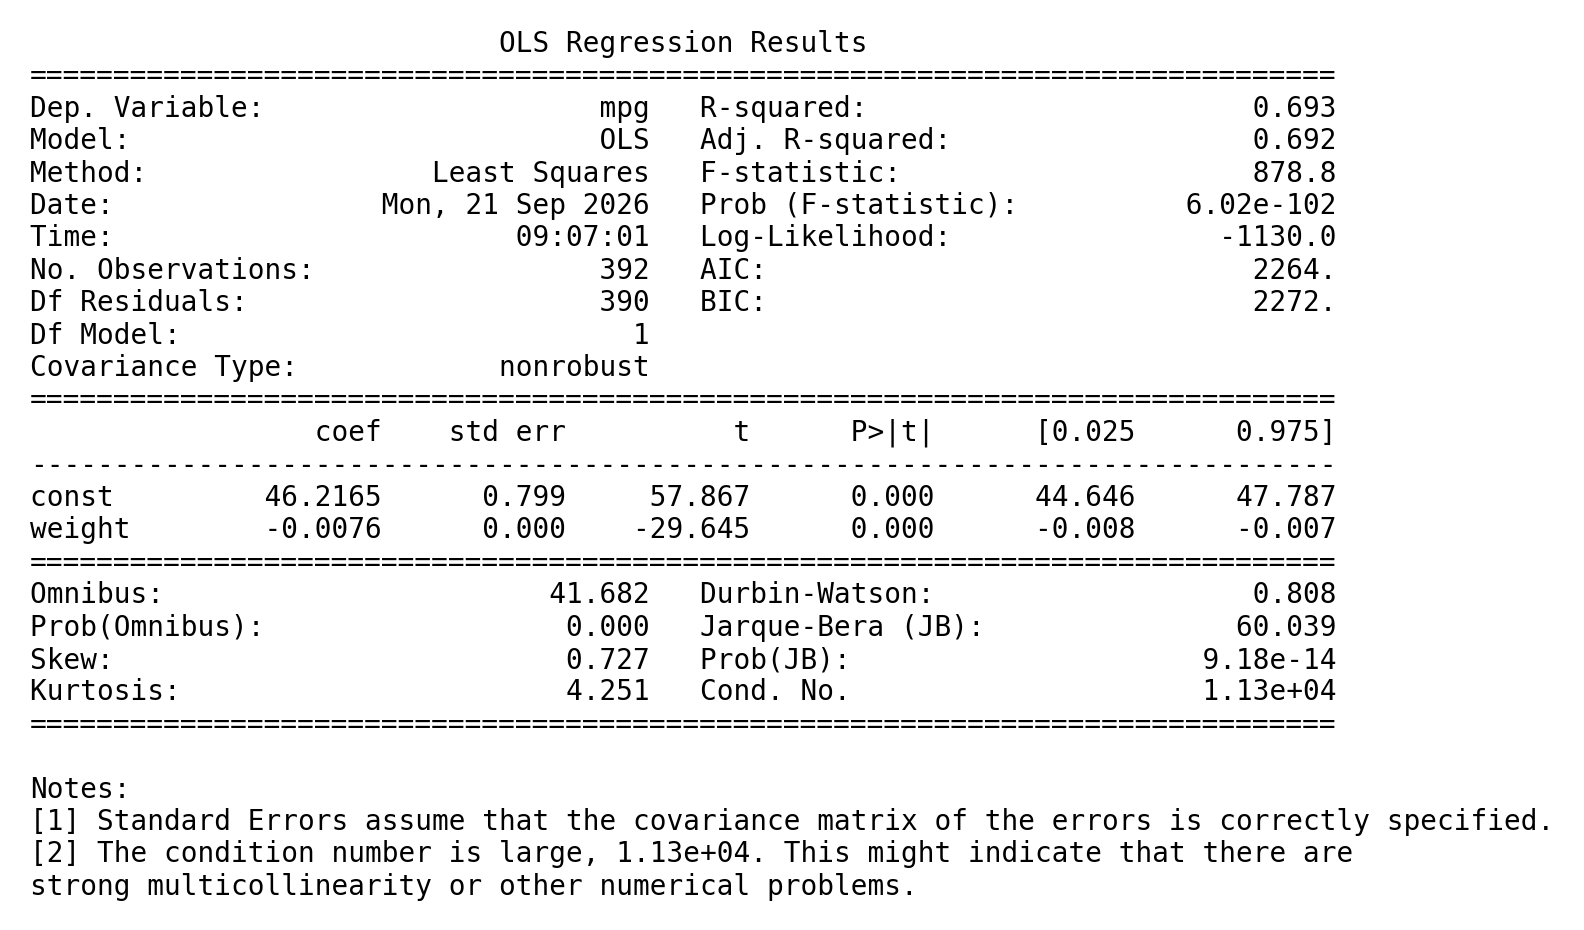
\includegraphics[width=0.45\textwidth]{MLR Figures/auto-MPG_weight_sr.png}
    \caption{Auto MPG simple regression using vehicle weight (\texttt{statsmodels} output).}
    \label{fig:auto-weight-simple}
\end{figure}

\begin{figure}[H]
    \centering
    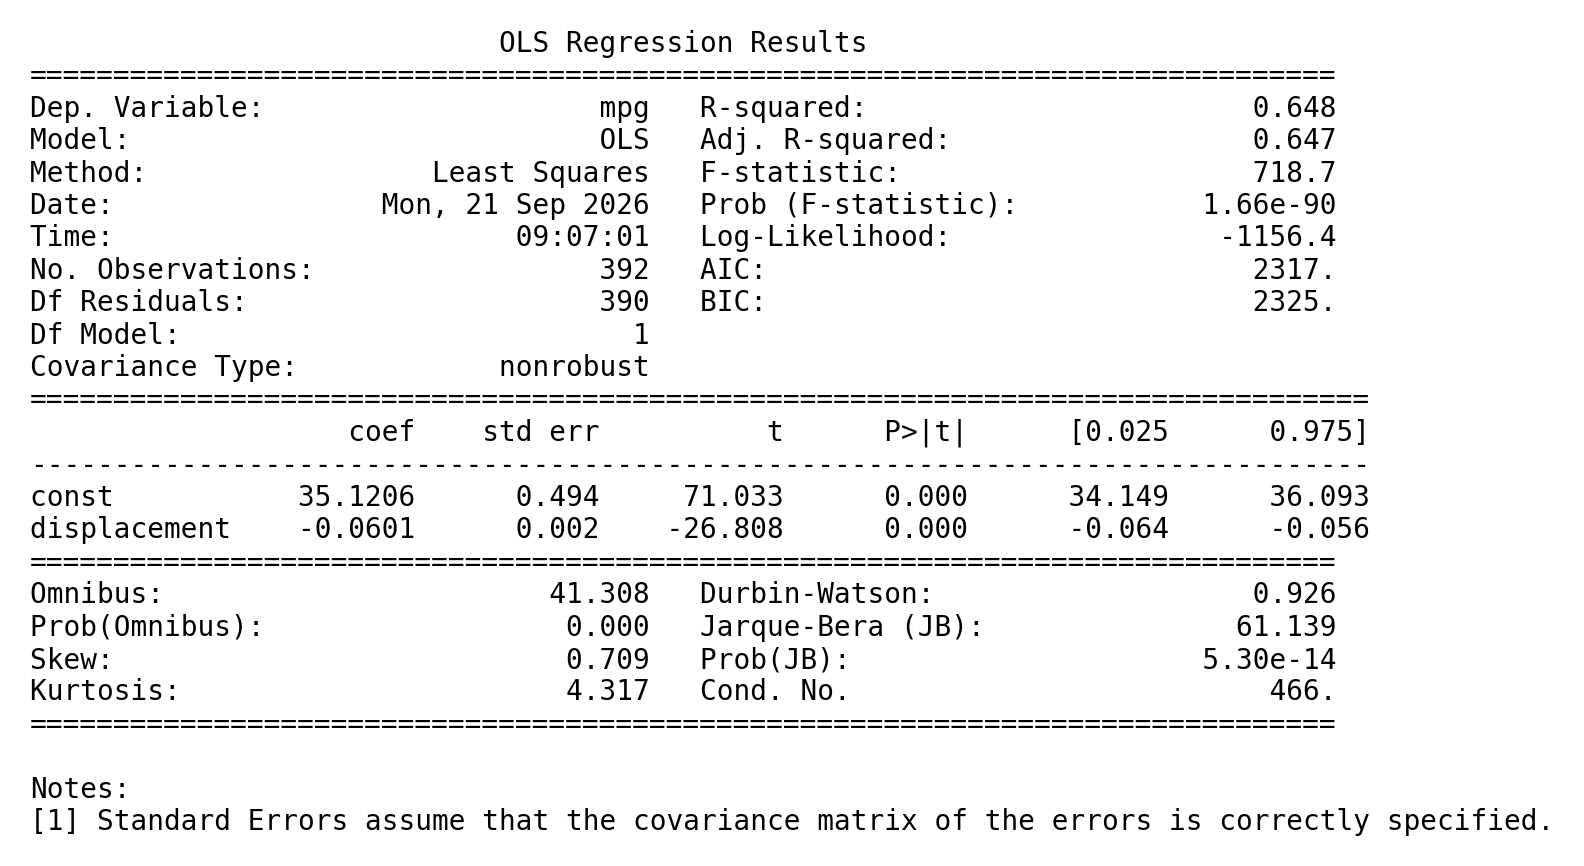
\includegraphics[width=0.45\textwidth]{MLR Figures/auto-MPG_displacement_sr.png}
    \caption{Auto MPG simple regression using vehicle displacement (\texttt{statsmodels} output).}
    \label{fig:auto-displacement-simple}
\end{figure}

\begin{figure}[H]
    \centering
    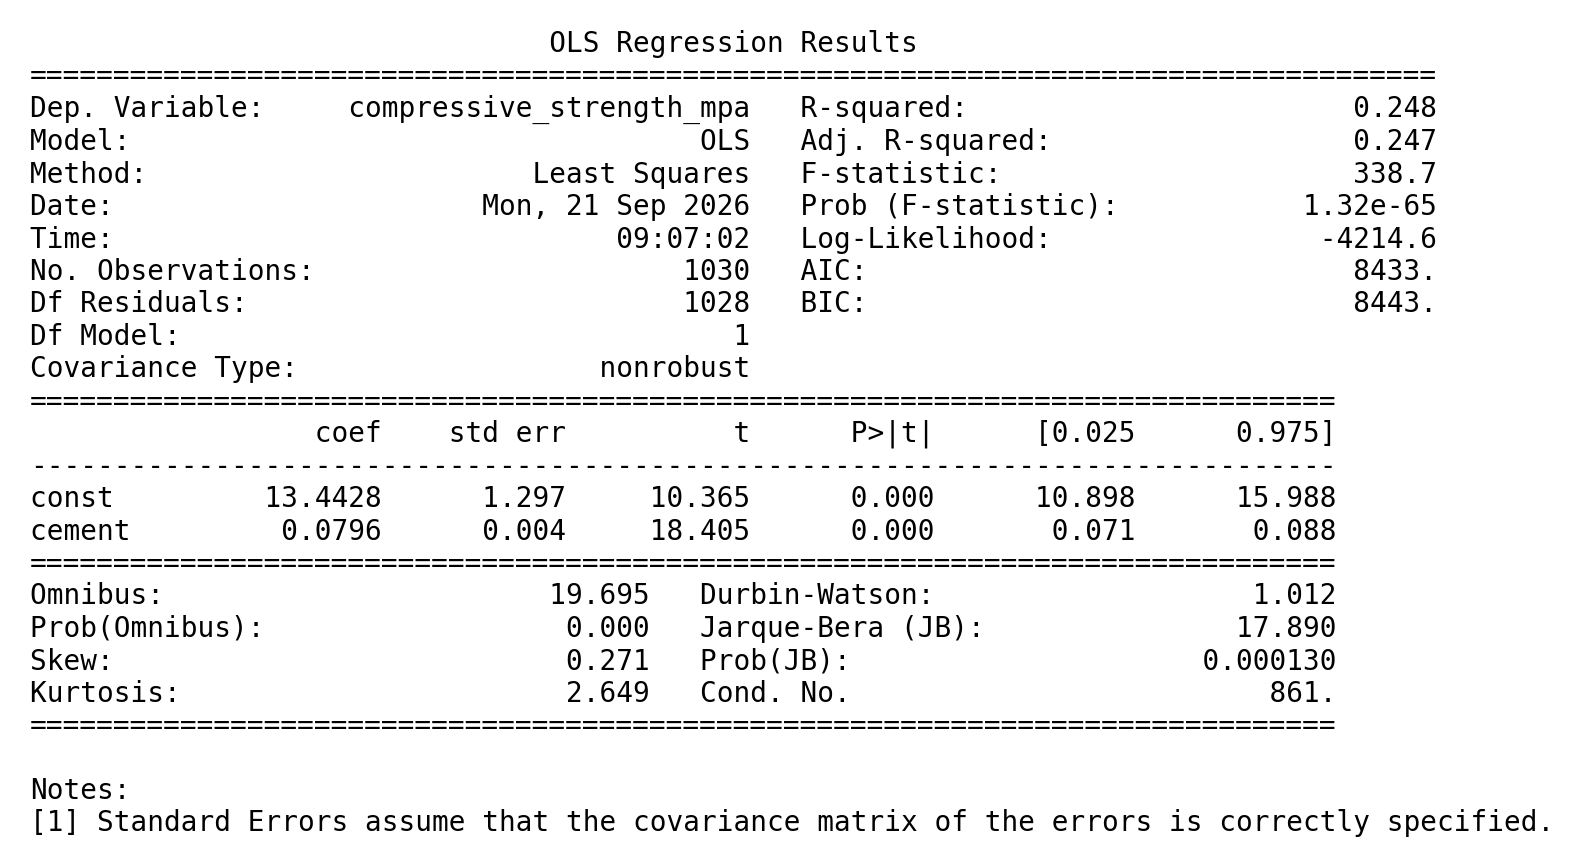
\includegraphics[width=0.45\textwidth]{MLR Figures/Concrete_cement_sr.png}
    \caption{Concrete simple regression using cement (\texttt{statsmodels} output).}
    \label{fig:concrete-cement-simple}
\end{figure}

\begin{figure}[H]
    \centering
    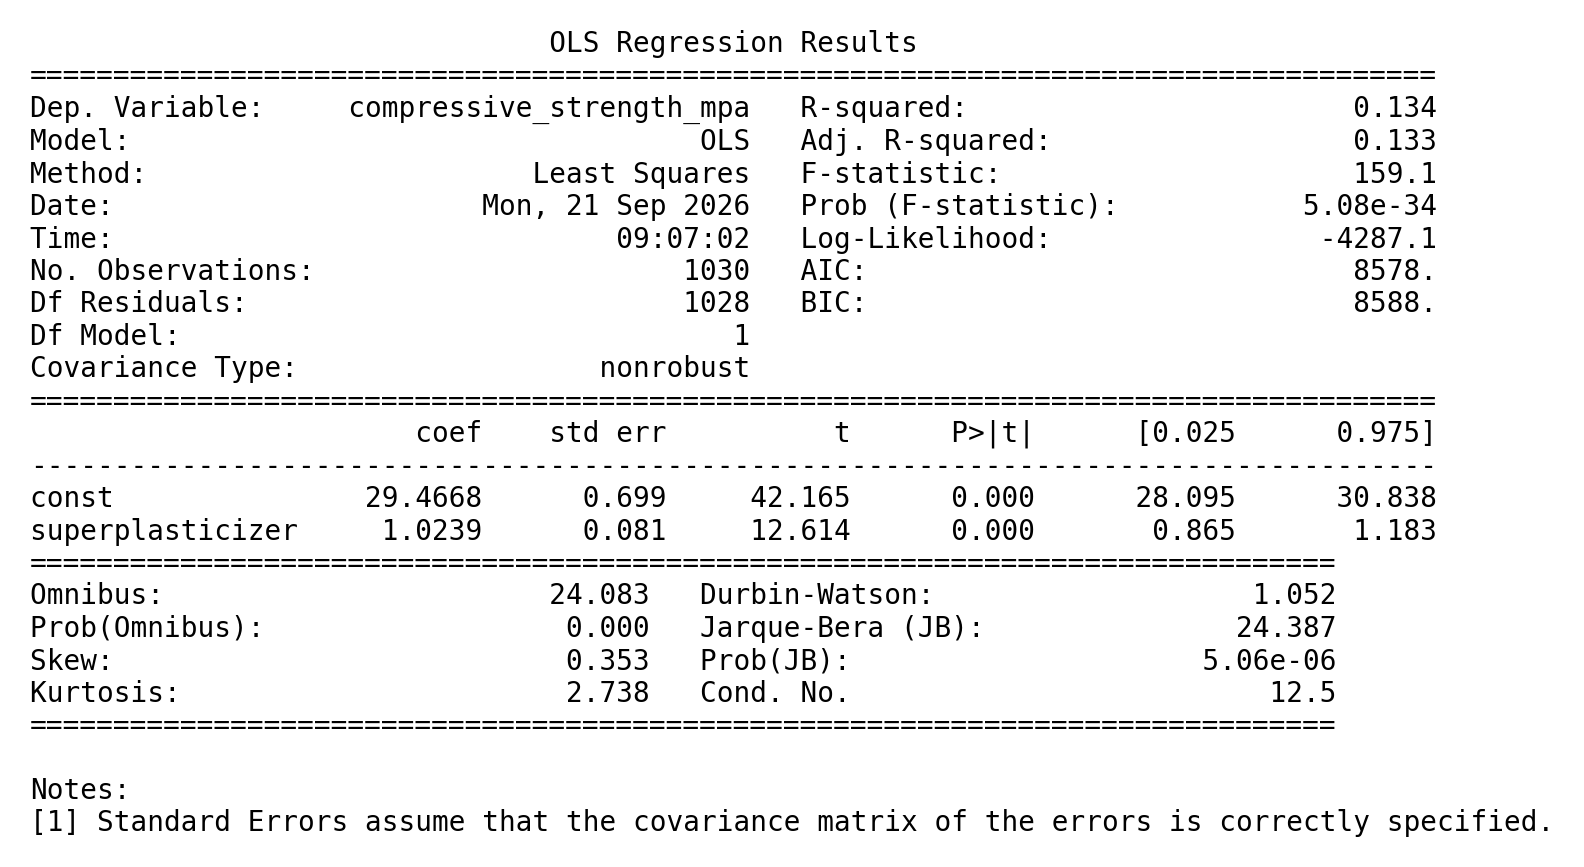
\includegraphics[width=0.45\textwidth]{MLR Figures/Concrete_sp_sr.png}
    \caption{Concrete simple regression using superplasticizer (\texttt{statsmodels} output).}
    \label{fig:concrete-superplasticizer-simple}
\end{figure}

\begin{figure}[H]
    \centering
    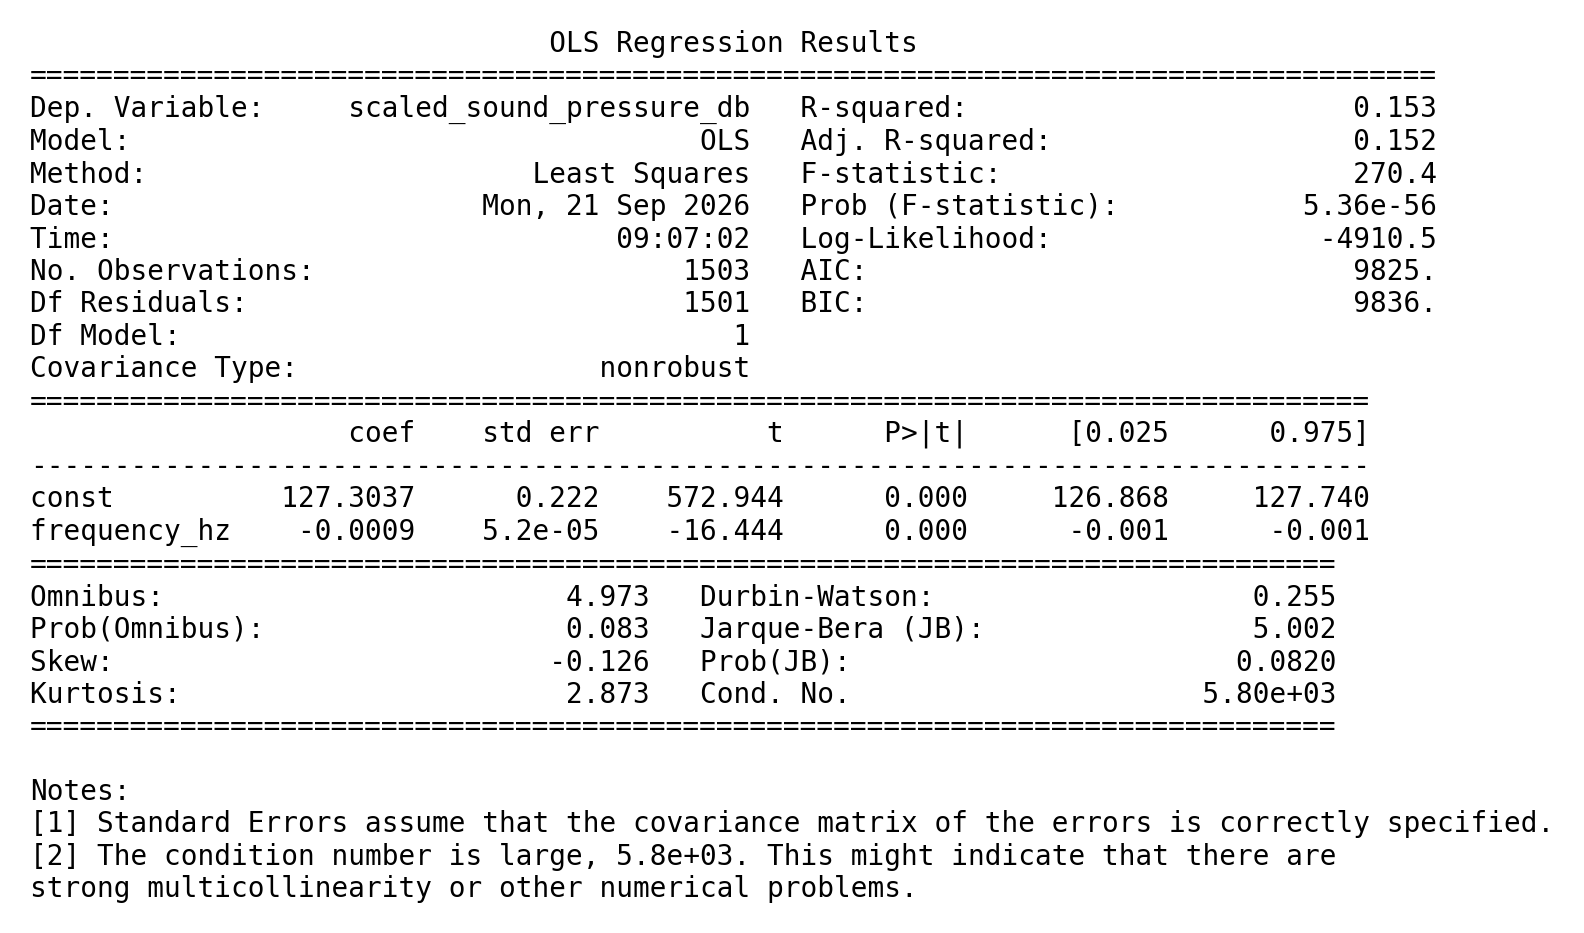
\includegraphics[width=0.45\textwidth]{MLR Figures/airfoil_frequency_sr.png}
    \caption{Airfoil simple regression using frequency (\texttt{statsmodels} output).}
    \label{fig:airfoil-frequency-simple}
\end{figure}

\begin{figure}[H]
    \centering
    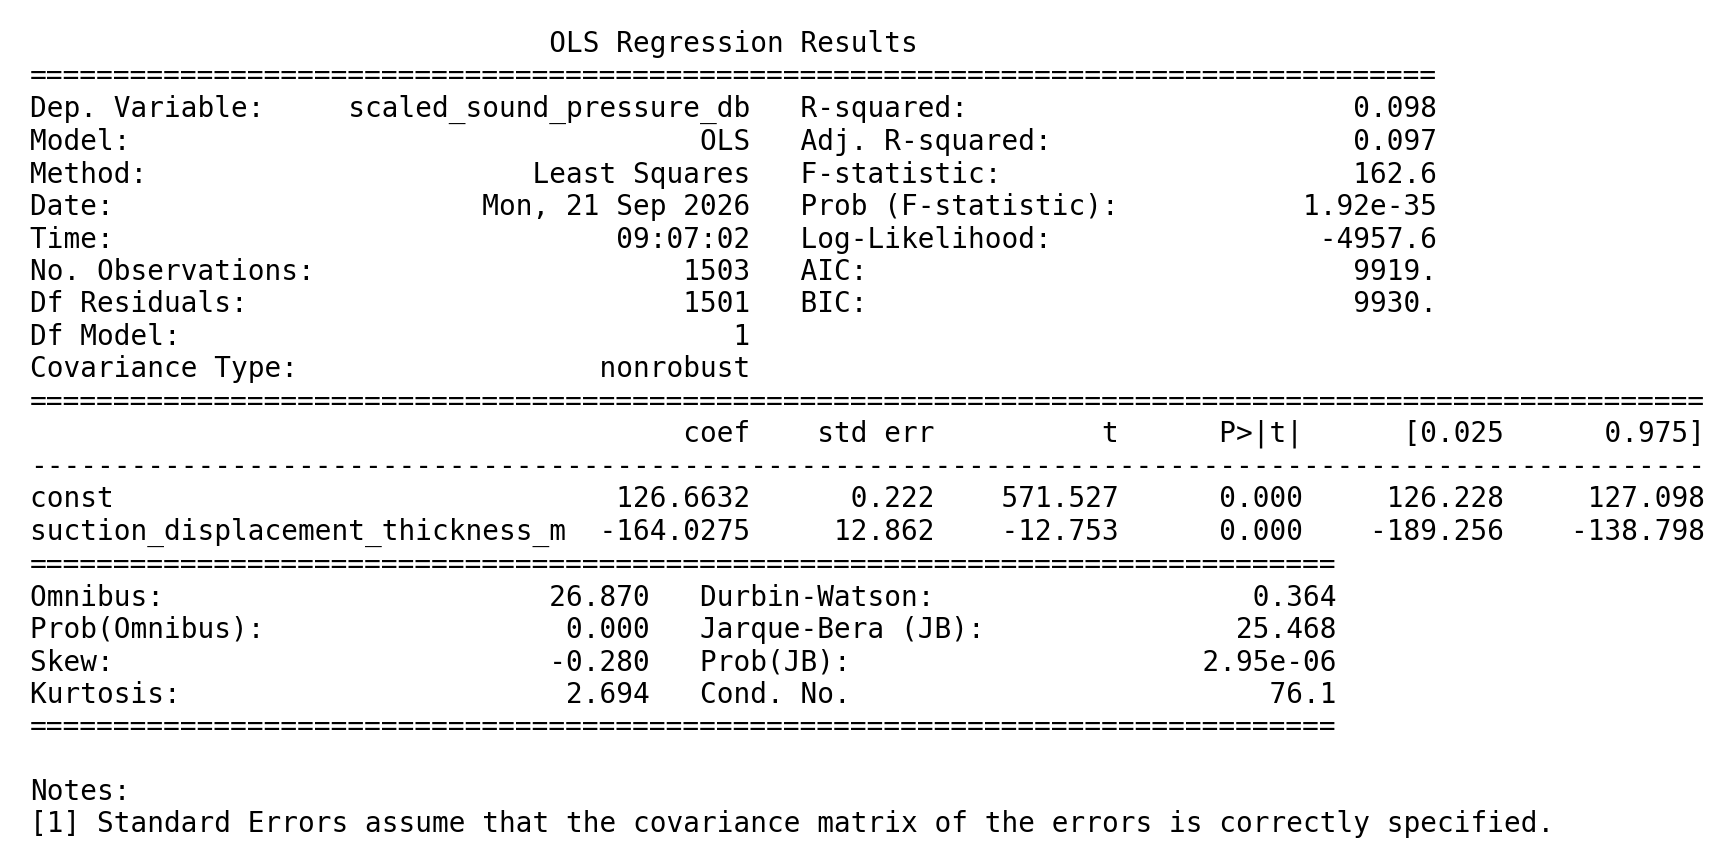
\includegraphics[width=0.45\textwidth]{MLR Figures/airfoil_displacement_sr.png}
    \caption{Airfoil simple regression using suction displacement thickness (\texttt{statsmodels} output).}
    \label{fig:airfoil-displacement-simple}
\end{figure}

\subsection{Results Comparison}

The ScalaTion and \texttt{statsmodels} implementations produced consistent results across all three datasets. Both implementations produced the same full-model $R^2$, adjusted $R^2$, residual standard error, and F-statistic to the displayed precision. The agreement between the two implementations is expected because both fit the same ordinary least squares multiple regression model using the same data and predictors.

For Auto MPG, the full model explained approximately 82.1\% of the variation in MPG. Weight had the largest absolute correlation with MPG among the predictors and produced a stronger simple regression fit than displacement. For Concrete, the full model explained approximately 61.5\% of the variation in compressive strength, while the individual simple regression models explained substantially less variation. For Airfoil, the full model explained approximately 51.6\% of the variation in scaled sound pressure, while the individual simple regression models explained less than 16\%.

The results also demonstrate the importance of considering relationships among predictors rather than evaluating coefficients independently. Auto MPG had particularly strong multicollinearity among cylinders, displacement, horsepower, and weight, while Concrete had moderate multicollinearity among several material composition variables. The Airfoil predictors showed comparatively lower multicollinearity. These differences help explain why the full regression models captured more variation in the response than the individual simple regressions, while multicollinearity made some individual coefficient estimates more difficult to interpret.



\subsection{Visual Comparison of the Fitted Models}

Figure~\ref{fig:mlr-simple-fits} shows the six simple regressions: the observed response $y$ and the fitted line $\hat{y}$ against each of the two most correlated predictors. Weight and displacement show clear downward trends for Auto MPG, while the Concrete and Airfoil predictors leave much more scatter around the fitted line, consistent with their lower $R^2$ values. The Auto MPG panels also show curvature: MPG falls steeply at low weight and displacement and levels off at high values, which a straight line cannot follow.

\begin{figure}[H]
\centering
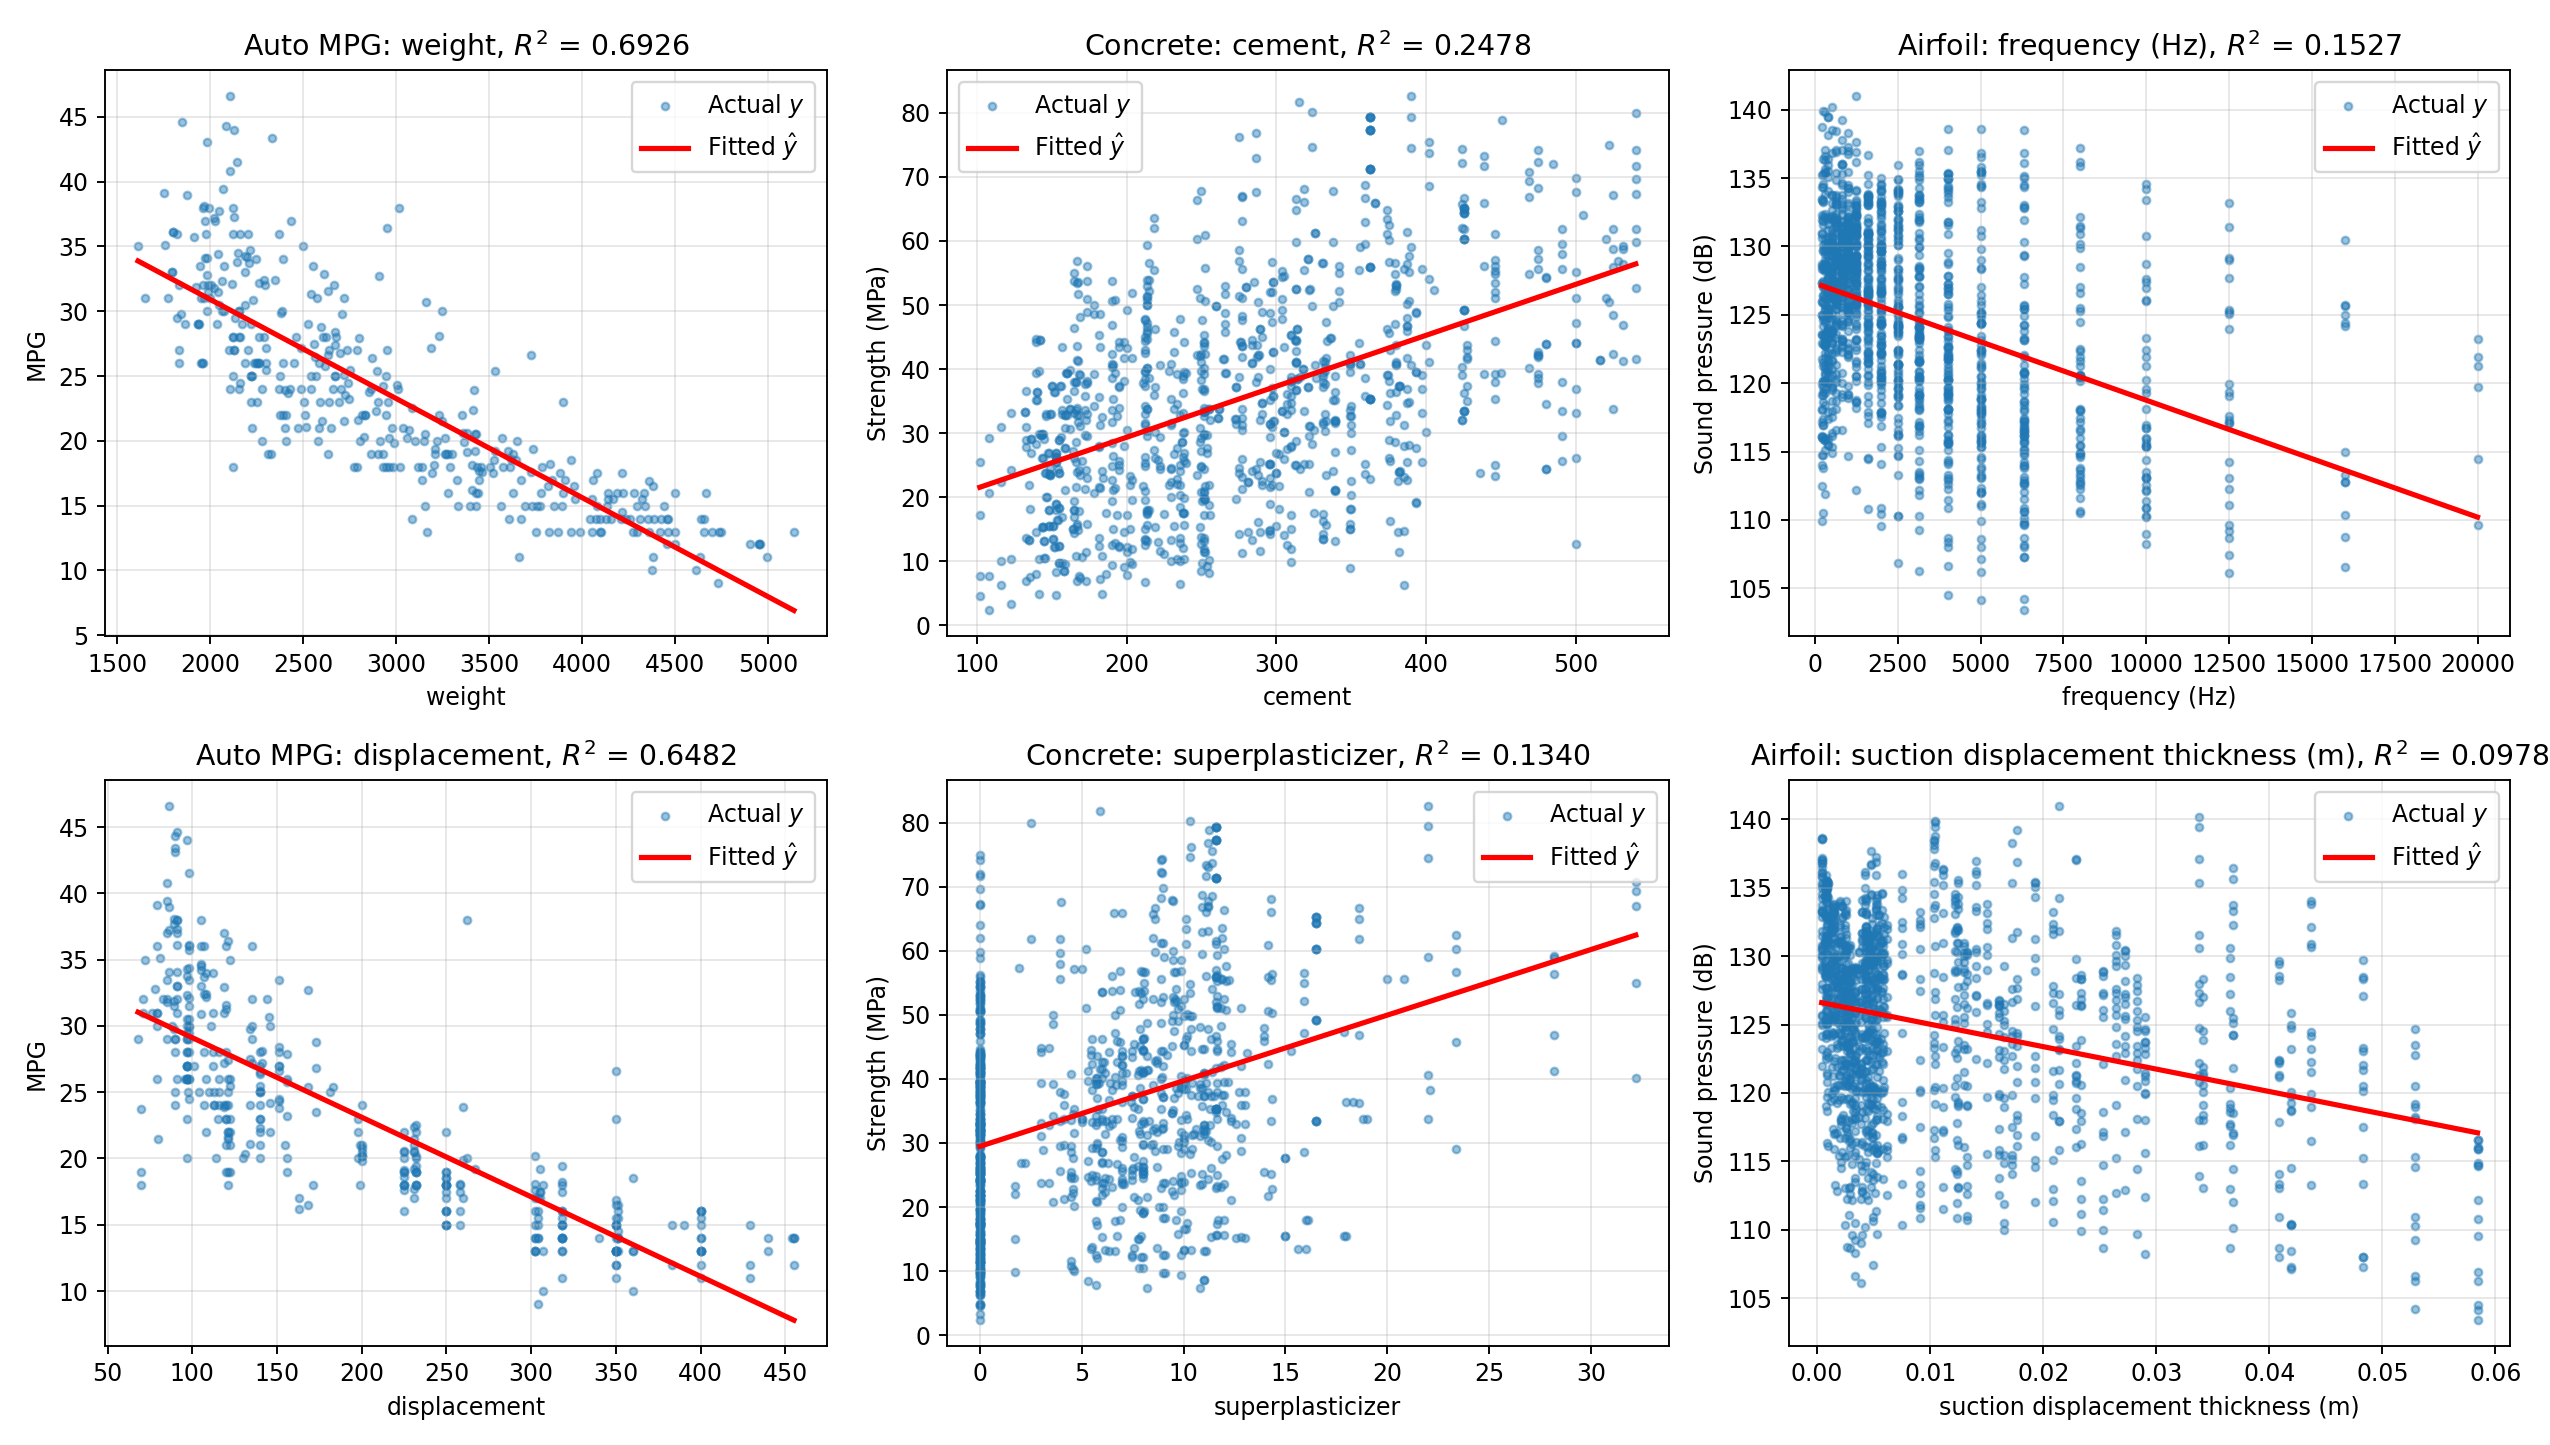
\includegraphics[width=\textwidth]{MLR Figures/simple_regression_fits.png}
\caption{Simple regression fits: observed $y$ and fitted $\hat{y}$ versus each of the two most correlated predictors for Auto MPG, Concrete, and Airfoil.}
\label{fig:mlr-simple-fits}
\end{figure}

Figure~\ref{fig:mlr-actual-pred} plots predicted against actual values for the three full multiple regression models. Auto MPG points lie close to the diagonal, although the highest-MPG cars are under-predicted. Concrete shows wider scatter around the diagonal. The Airfoil predictions are compressed toward the middle of the range: the model over-predicts the quietest observations and under-predicts the loudest, which reflects its lower $R^2$ of 0.516.

\begin{figure}[H]
\centering
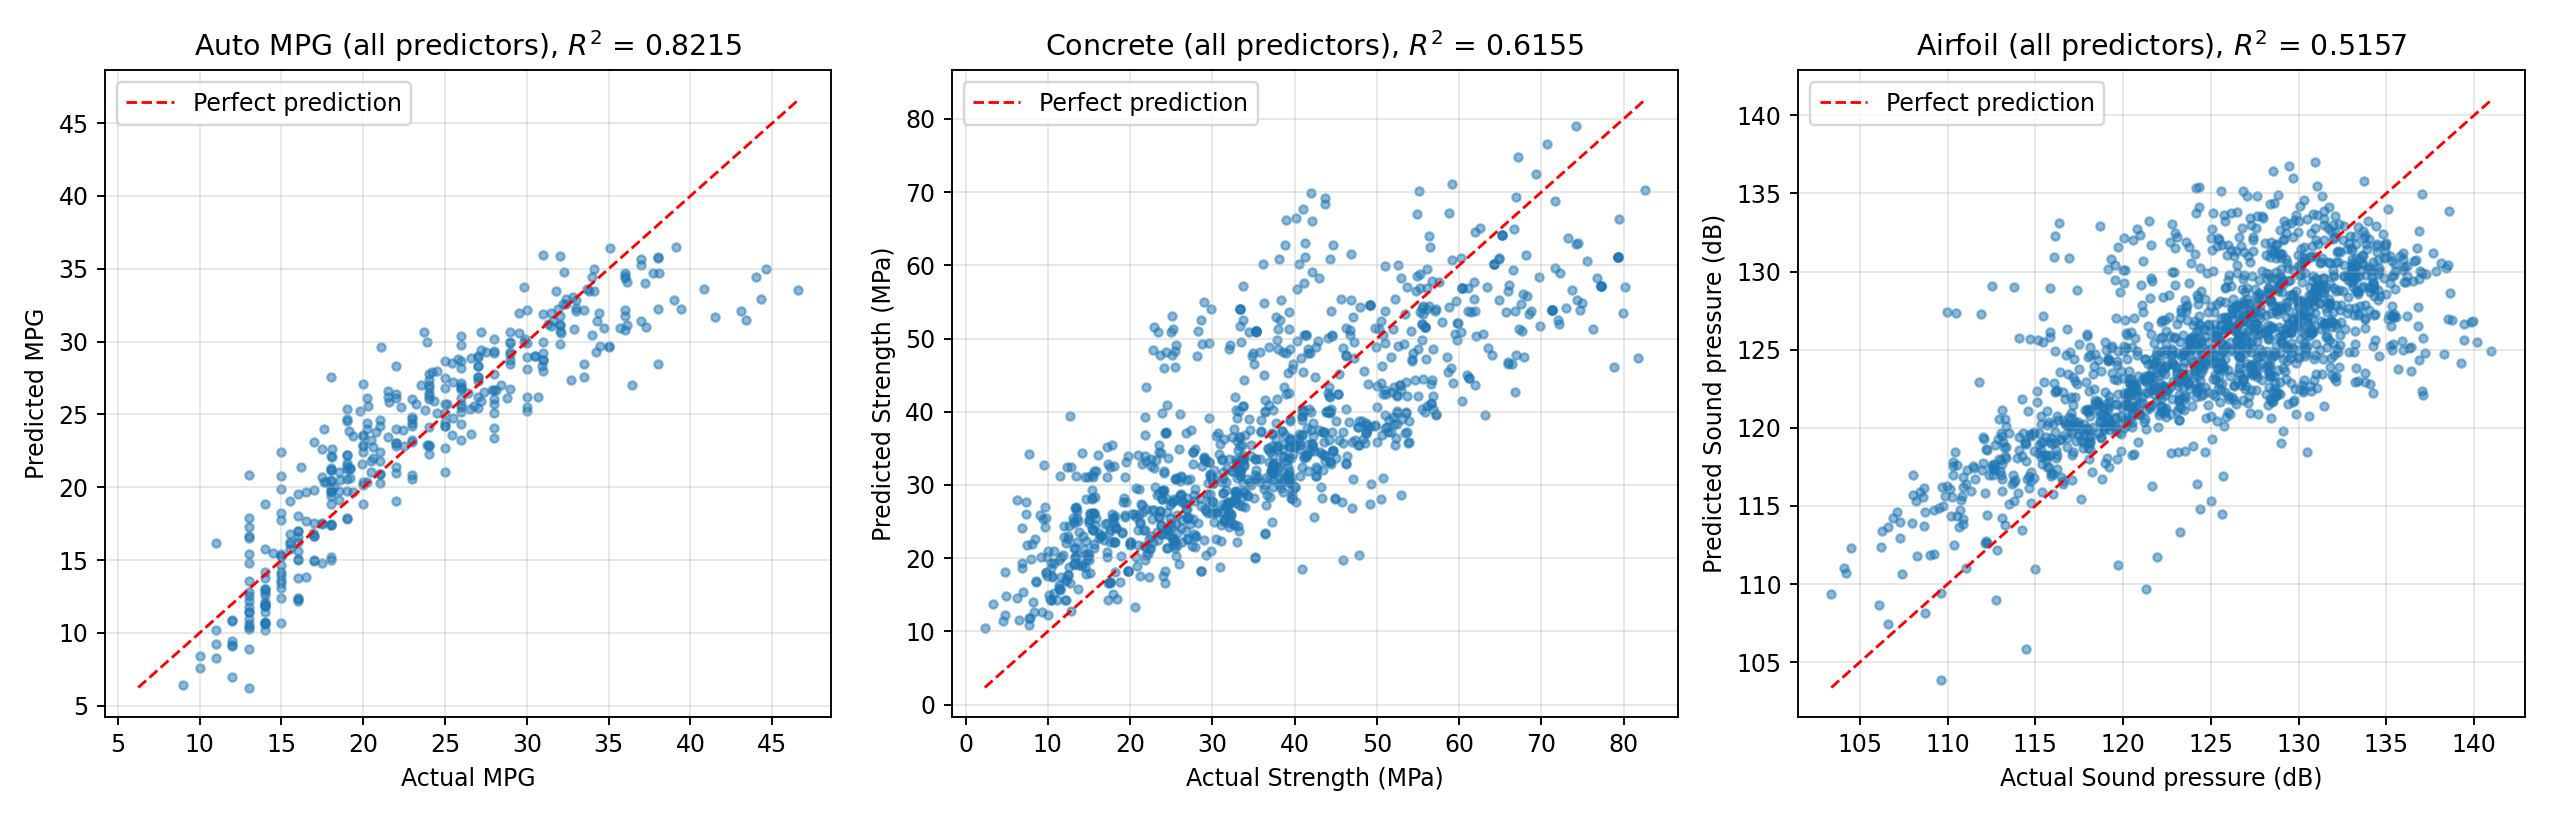
\includegraphics[width=\textwidth]{MLR Figures/full_model_actual_vs_predicted.png}
\caption{Predicted versus actual values for the full multiple regression models (in-sample). The dashed line marks perfect prediction.}
\label{fig:mlr-actual-pred}
\end{figure}

\section{Regularized Regression}

Ridge and Lasso were fitted to Auto MPG in both ScalaTion and \texttt{statsmodels}, giving four required cases. Ridge penalizes squared slope coefficients; Lasso penalizes their absolute values and can yield sparse models. Both implementations standardize predictors using training statistics and leave the intercept unpenalized. Origin is retained as a numeric predictor, matching the multiple regression setup.

\subsection{statsmodels}

The notebook uses a scikit-learn seed-42 80/20 split (313 training, 79 test rows). Five-fold CV with shuffled seed-42 folds considers $\alpha\in\{0.001,0.01,0.1,1,10,100\}$. A new scaler is fitted inside each fold, and the intercept has zero penalty weight. The tuning score is mean fold RMSE. Both methods select $\alpha=0.01$. Final scalers and coefficients are fitted using the complete training set, then evaluated once on test data.

\subsection{ScalaTion}

The ScalaTion implementation uses Scala's seed-42 shuffle (314 training, 78 test rows). For both methods, five contiguous folds of the shuffled training rows evaluate the same grid $\lambda=0.1\,2^i$, $i=0,\ldots,19$. Each fold estimates predictor means and sample standard deviations, and centers the response, using only its fitting rows. Validation predictions add that fold's response mean back. Lambda minimizes pooled CV RMSE, $\sqrt{\sum e_i^2/n_{train}}$. The final model uses complete-training statistics and adds the training response mean back, so the intercept is unpenalized.

\begin{table}[H]
\centering\small
\caption{Auto MPG Ridge and Lasso test-set results. The two tools use different test rows.}
\label{tab:regularized-results}
\begin{tabular}{lllrr}
\toprule
Tool & Method & Penalty & Test RMSE & Test $R^2$ \\
\midrule
statsmodels & Ridge & $\alpha=0.01$ & 3.2973 & 0.7870 \\
ScalaTion & Ridge & $\lambda=0.8$ & 3.5348 & 0.7826 \\
statsmodels & Lasso & $\alpha=0.01$ & 3.2907 & 0.7878 \\
ScalaTion & Lasso & $\lambda=0.8$ & 3.5295 & 0.7832 \\
\bottomrule
\end{tabular}
\end{table}

\begin{table}[H]
\centering\small
\caption{Coefficients on standardized predictors; intercepts are in MPG. Each tool uses its own training scaler.}
\label{tab:regularized-coefficients}
\begin{tabular}{lrrrr}
\toprule
Term & SM Ridge & SM Lasso & Scala Ridge & Scala Lasso \\
\midrule
intercept & 23.599361 & 23.599361 & 23.416561 & 23.416561 \\
cylinders & -0.469692 & -0.382769 & -1.177008 & -1.177037 \\
displacement & 0.977049 & 1.128755 & 1.726830 & 1.824915 \\
horsepower & -0.908489 & -0.839027 & -0.469544 & -0.421403 \\
weight & -4.667132 & -4.975586 & -5.145695 & -5.274320 \\
acceleration & 0.006313 & 0.000000 & 0.091504 & 0.118477 \\
model year & 2.722611 & 2.764608 & 2.697029 & 2.710472 \\
origin & 1.268601 & 1.258881 & 1.161311 & 1.159458 \\
\bottomrule
\end{tabular}
\end{table}

Weight has a large negative coefficient and model year a positive coefficient in all four fitted models. statsmodels Lasso sets acceleration exactly to zero. The Scala Lasso keeps a small nonzero acceleration coefficient; sparsity depends on the chosen penalty and solver tolerance. Because these are coefficients on standardized, correlated predictors, their signs describe conditional fitted associations rather than independent causal effects. Ridge penalization discourages large slope estimates among correlated cylinders, displacement, horsepower, and weight, allowing their shared information to remain in the fitted model. Lasso can remove a redundant predictor, as with acceleration in \texttt{statsmodels}; a zero conditional coefficient does not establish that the variable has no marginal association with MPG.

\subsection{Evaluation and Interpretation}

On the statsmodels test split, unregularized OLS has RMSE 3.2727~MPG; on the ScalaTion split it has RMSE 3.5276~MPG. The regularized fits do not improve test RMSE over these matched-split baselines. Regularization shrinks coefficients and can reduce variance in other samples, but this experiment does not demonstrate reduced overfitting. Alpha and lambda values cannot be compared numerically across implementations because their penalty normalizations differ. Differences between tools also reflect different test rows, scaler conventions, solvers, and tuning objectives. The two tuning scores are mean fold RMSE (statsmodels) and pooled RMSE (ScalaTion); neither is a test-set score.

\begin{figure}[H]
\centering
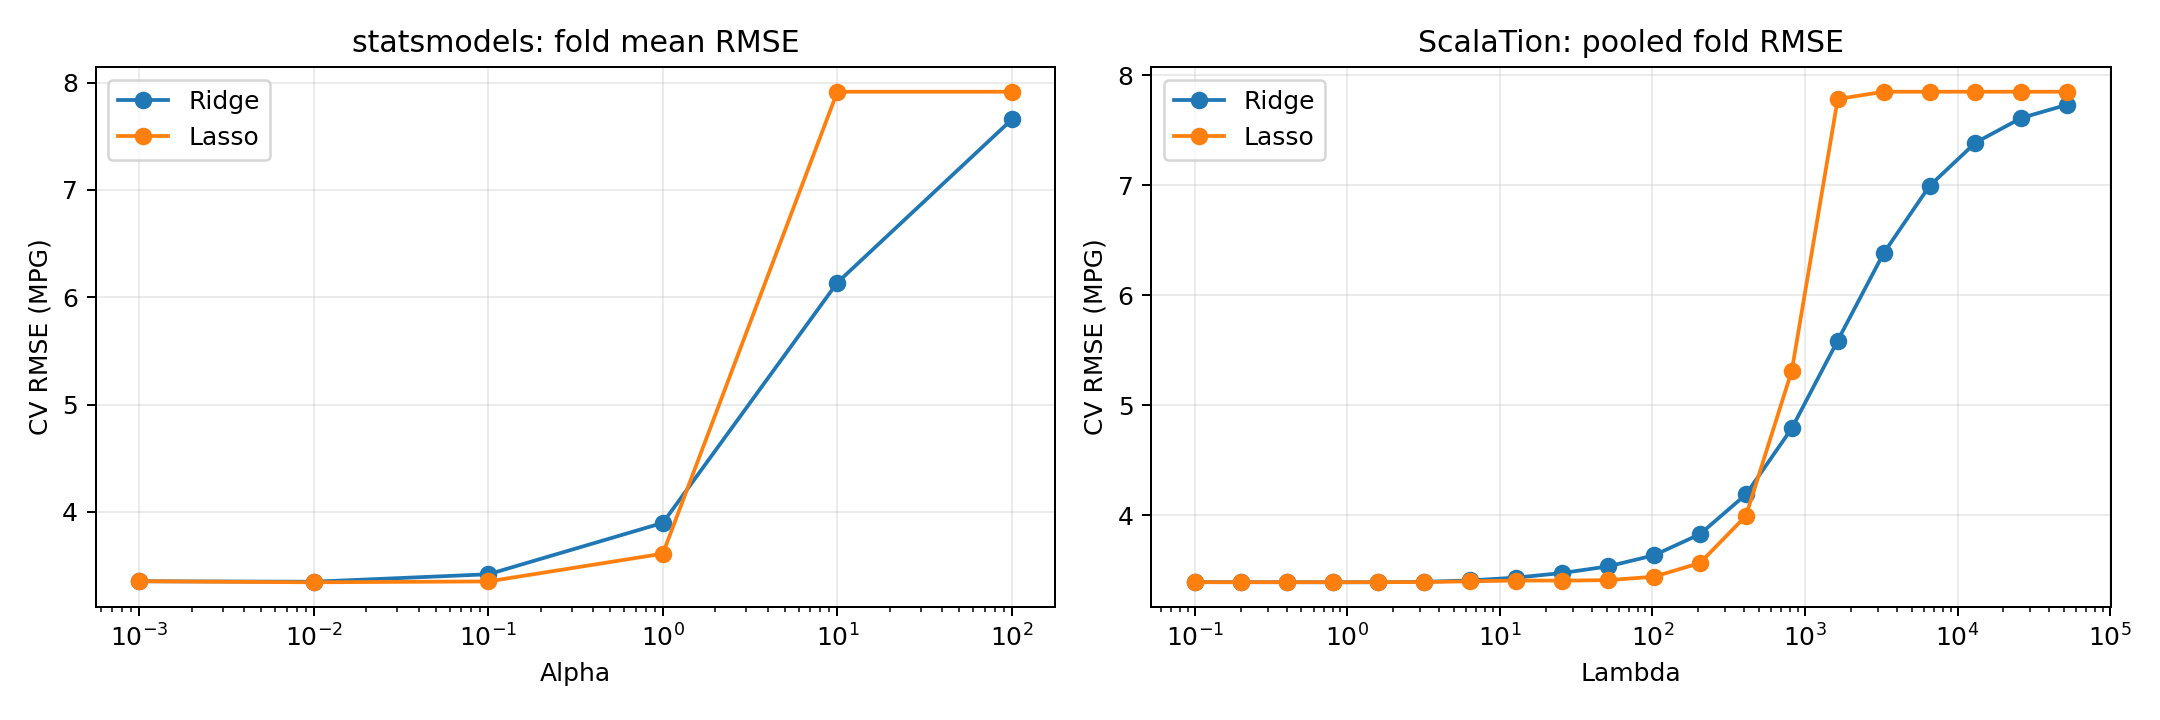
\includegraphics[width=\textwidth]{Regular Regression Images/tuning_comparison.png}
\caption{Training CV tuning curves for Ridge and Lasso. Each candidate in the ScalaTion curves uses the same folds and fold-specific preprocessing.}
\label{fig:reg-tuning}
\end{figure}

\begin{figure}[H]
\centering
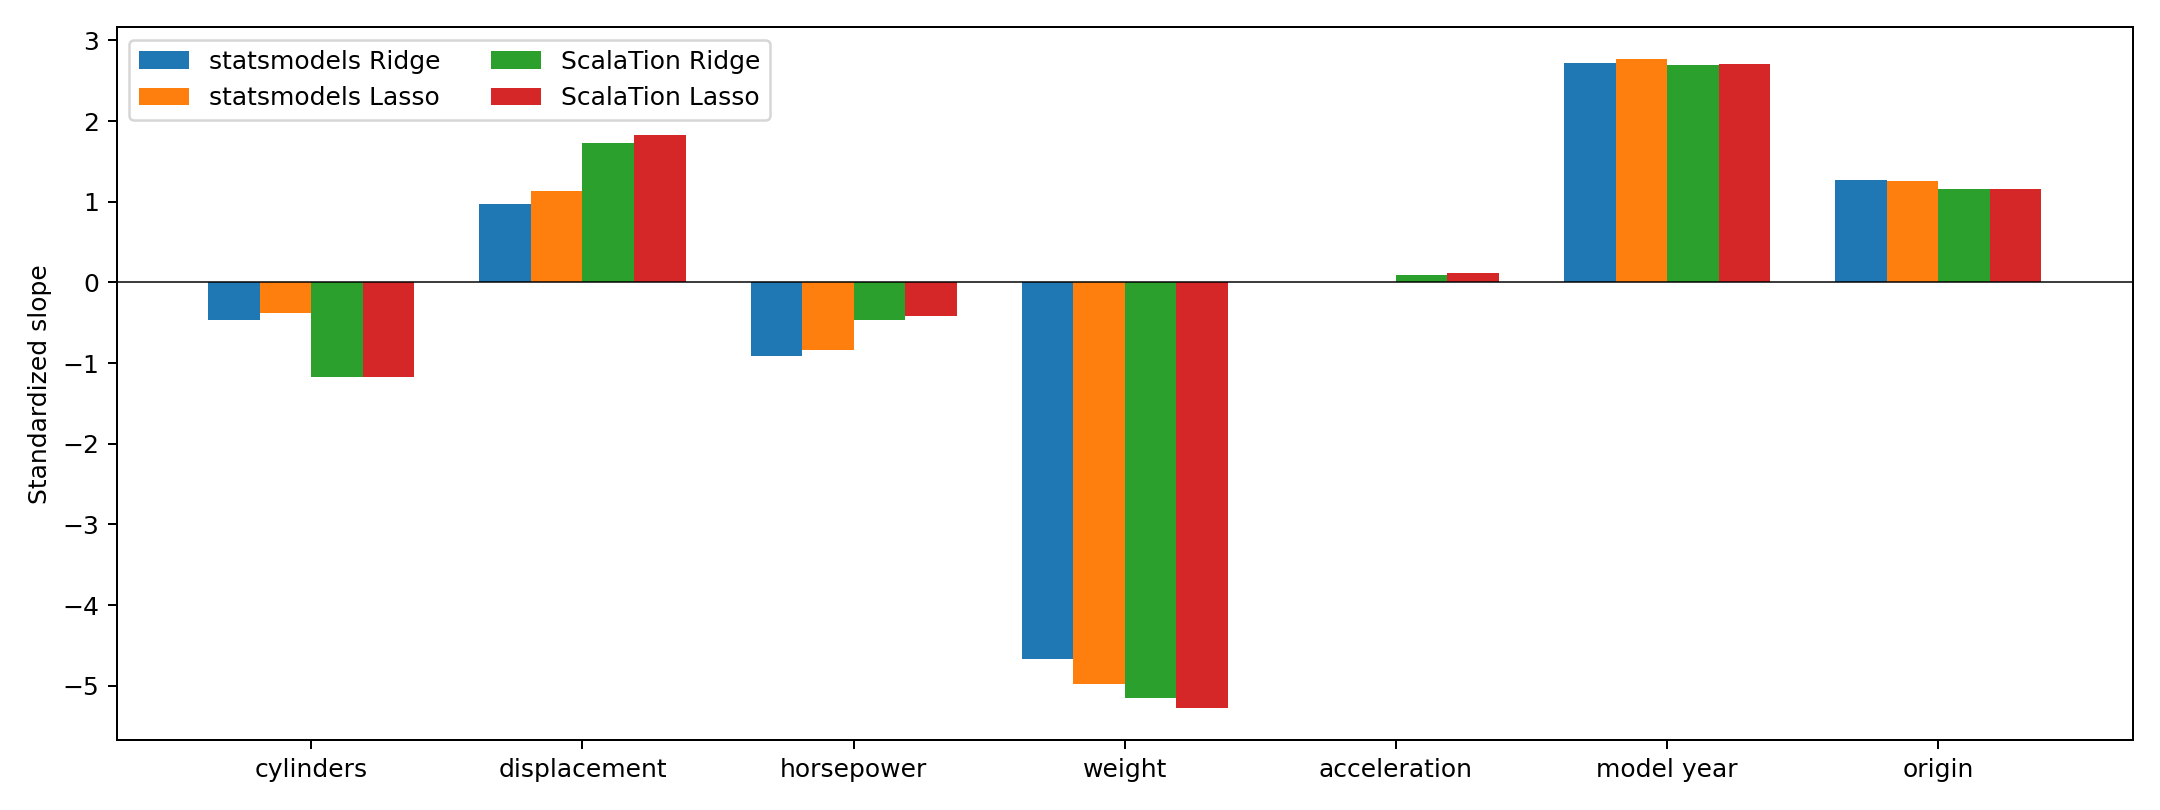
\includegraphics[width=\textwidth]{Regular Regression Images/coefficient_comparison.png}
\caption{Ridge/Lasso slope coefficients on standardized predictors for all four Auto MPG models.}
\label{fig:reg-coef}
\end{figure}

\begin{figure}[H]
\centering
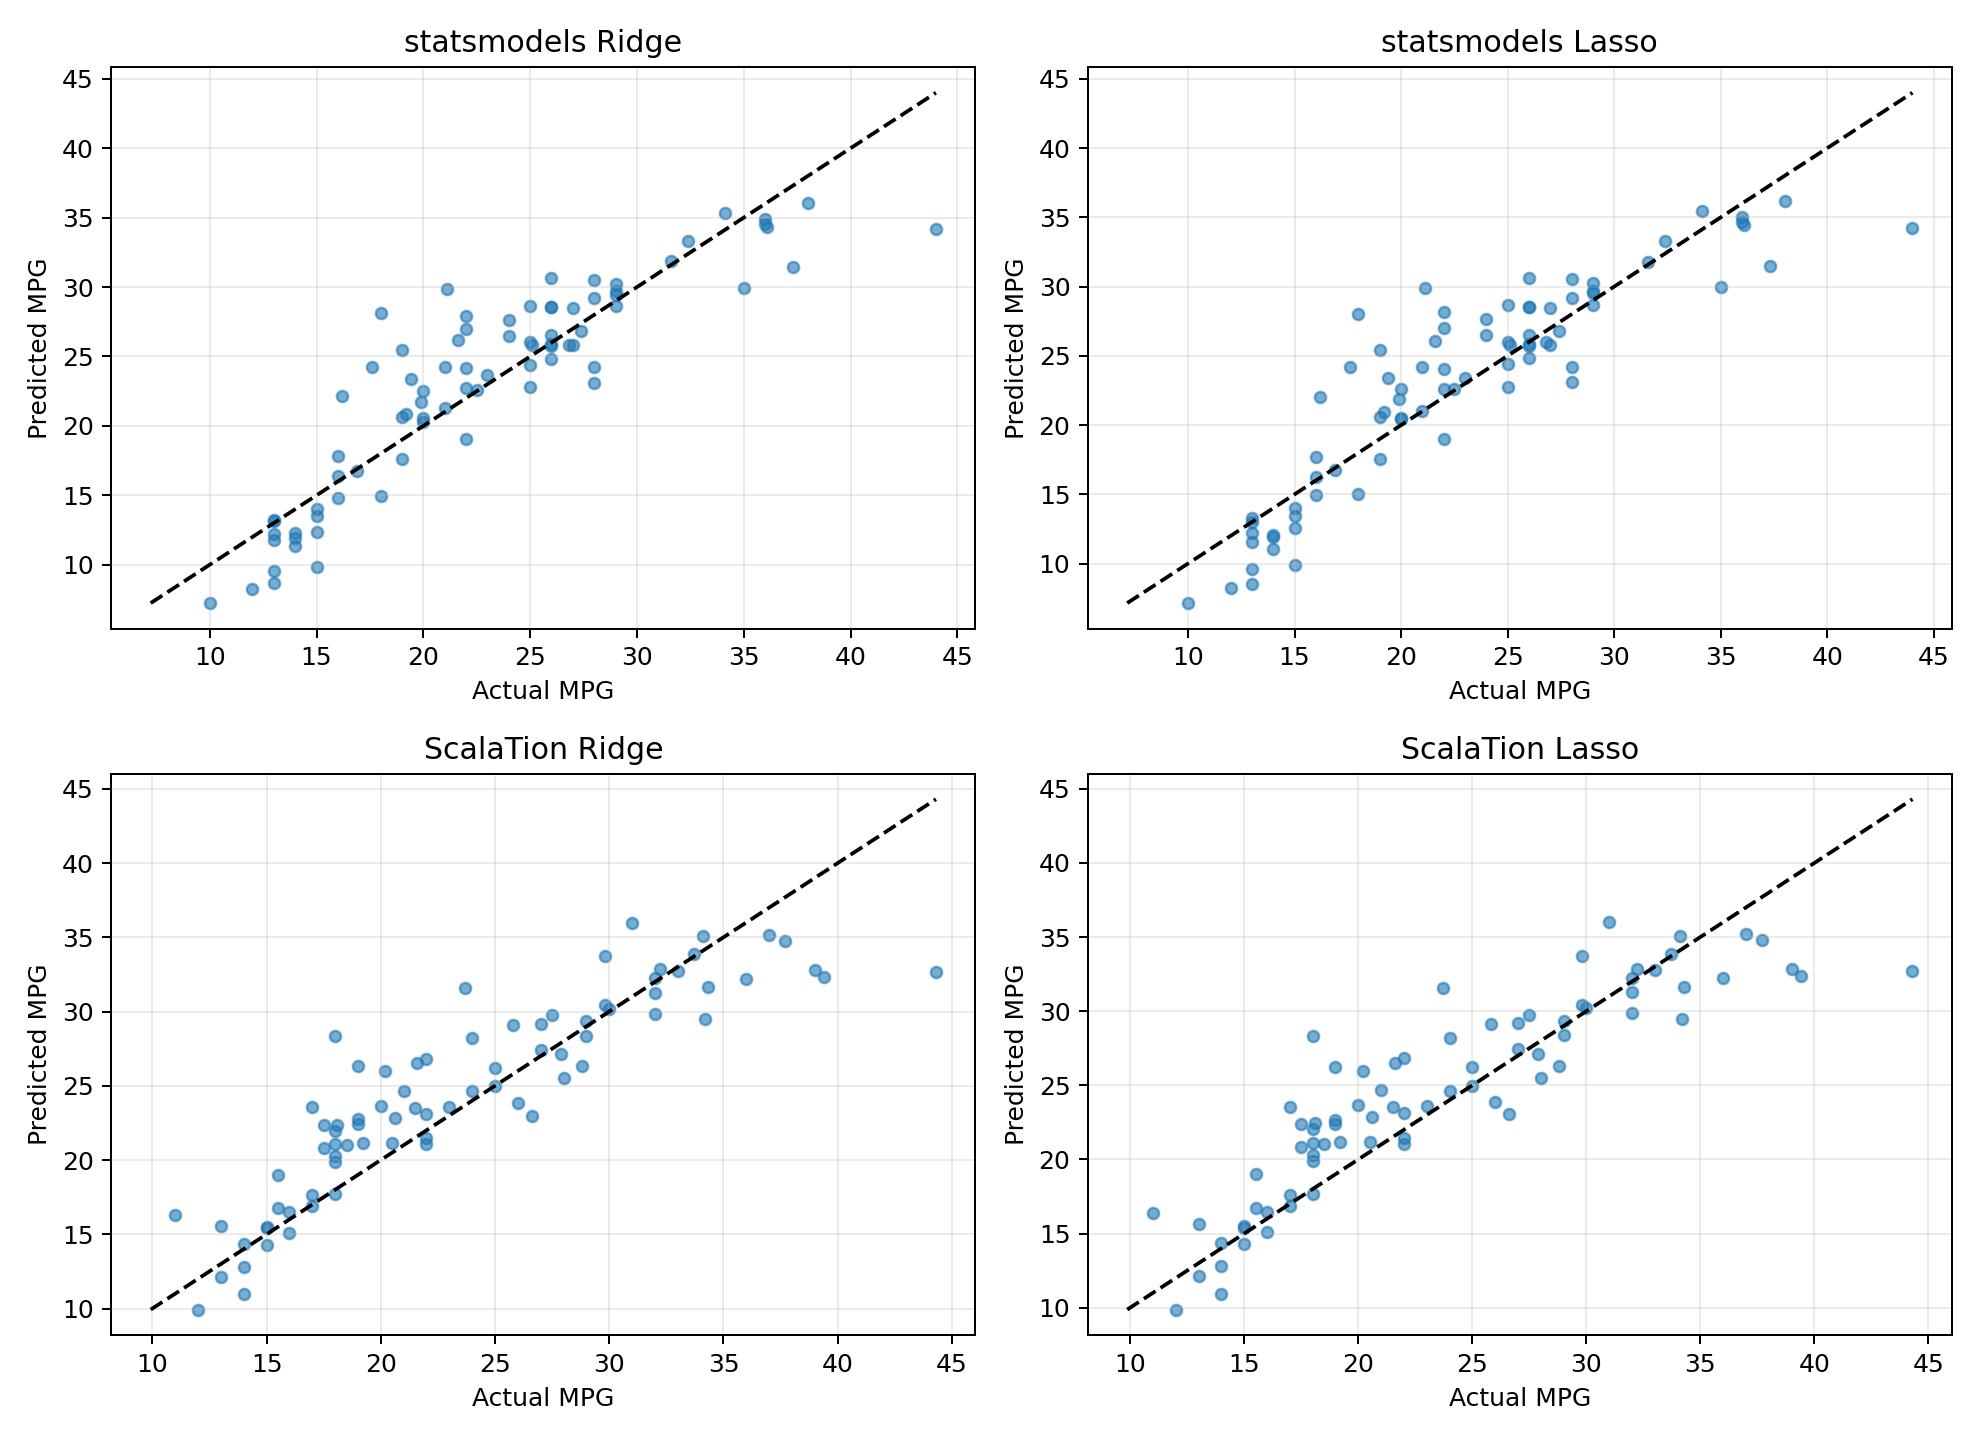
\includegraphics[width=\textwidth]{Regular Regression Images/test_actual_vs_predicted.png}
\caption{Observed versus predicted test MPG. Each ScalaTion panel uses the coefficients and untouched outer test rows; statsmodels uses its own split.}
\label{fig:reg-test}
\end{figure}

\section{Forward Feature Selection}

Forward feature selection was run in ScalaTion on two datasets, Auto MPG ($n = 392$) and Concrete ($n = 1{,}030$). For each dataset, the rows were shuffled once with a fixed random seed (42), and a multiple regression model with an intercept column was built over the available predictors. ScalaTion's \texttt{forwardSelAll} routine then started from an intercept-only model and added one variable at a time, at each step choosing the addition that maximized adjusted $R^2$ (\texttt{QoF.rSqBar}). At steps 1 onward, candidate models were fitted on ScalaTion's default training range (313 rows for Auto MPG and 823 for Concrete), so the path $R^2$ and adjusted $R^2$ values are training-set measures; adjusted $R^2$ was recomputed with the training-set size, because \texttt{forwardSelAll} reports it using the full dataset size. The intercept-only step is fitted on the full dataset. Each candidate subset was also evaluated with the default 5-fold cross-validation on the full dataset, so $R^2_{cv}$ is the average out-of-sample $R^2$ across the five folds. The best model is the step where adjusted $R^2$ is maximized over the full selection path, and that subset of variables was refit with \texttt{trainNtest()} on the full dataset.

\subsection{ScalaTion}

\subsubsection{Auto MPG}

Forward selection considered the seven predictors (cylinders, displacement, horsepower, weight, acceleration, model year, and origin) for MPG. Table~\ref{tab:fs-auto-path} lists the variable added at each step along with the metrics reported by \texttt{forwardSelAll} (all values in \%), and Figure~\ref{fig:fs-auto-path} plots them against the number of predictors.

\begin{table}[H]
    \centering
    \caption{Forward selection path for Auto MPG (values in \%). Adjusted $R^2$ peaks at step 6. Adjusted $R^2$ is computed with the training-set size used by \texttt{forwardSelAll} (313 rows).}
    \label{tab:fs-auto-path}
    \begin{tabular}{clcccc}
        \hline
        Step & Variable added & $R^2$ & Adjusted $R^2$ & sMAPE & $R^2_{cv}$ \\
        \hline
        0 & intercept & $-0.000$ & $0.00$ & 28.410 & $-1.283$ \\
        1 & weight & 70.660 & 70.57 & 13.919 & 68.892 \\
        2 & model year & 81.461 & 81.34 & 11.867 & 80.384 \\
        3 & origin & 82.532 & 82.36 & 11.187 & 80.984 \\
        4 & cylinders & 82.583 & 82.36 & 11.113 & 80.784 \\
        5 & displacement & 82.779 & 82.50 & 11.068 & 80.851 \\
        6 & horsepower & 82.856 & \textbf{82.52} & 11.173 & 81.063 \\
        7 & acceleration & 82.866 & 82.47 & 11.187 & 80.855 \\
        \hline
    \end{tabular}
\end{table}

\begin{figure}[H]
    \centering
    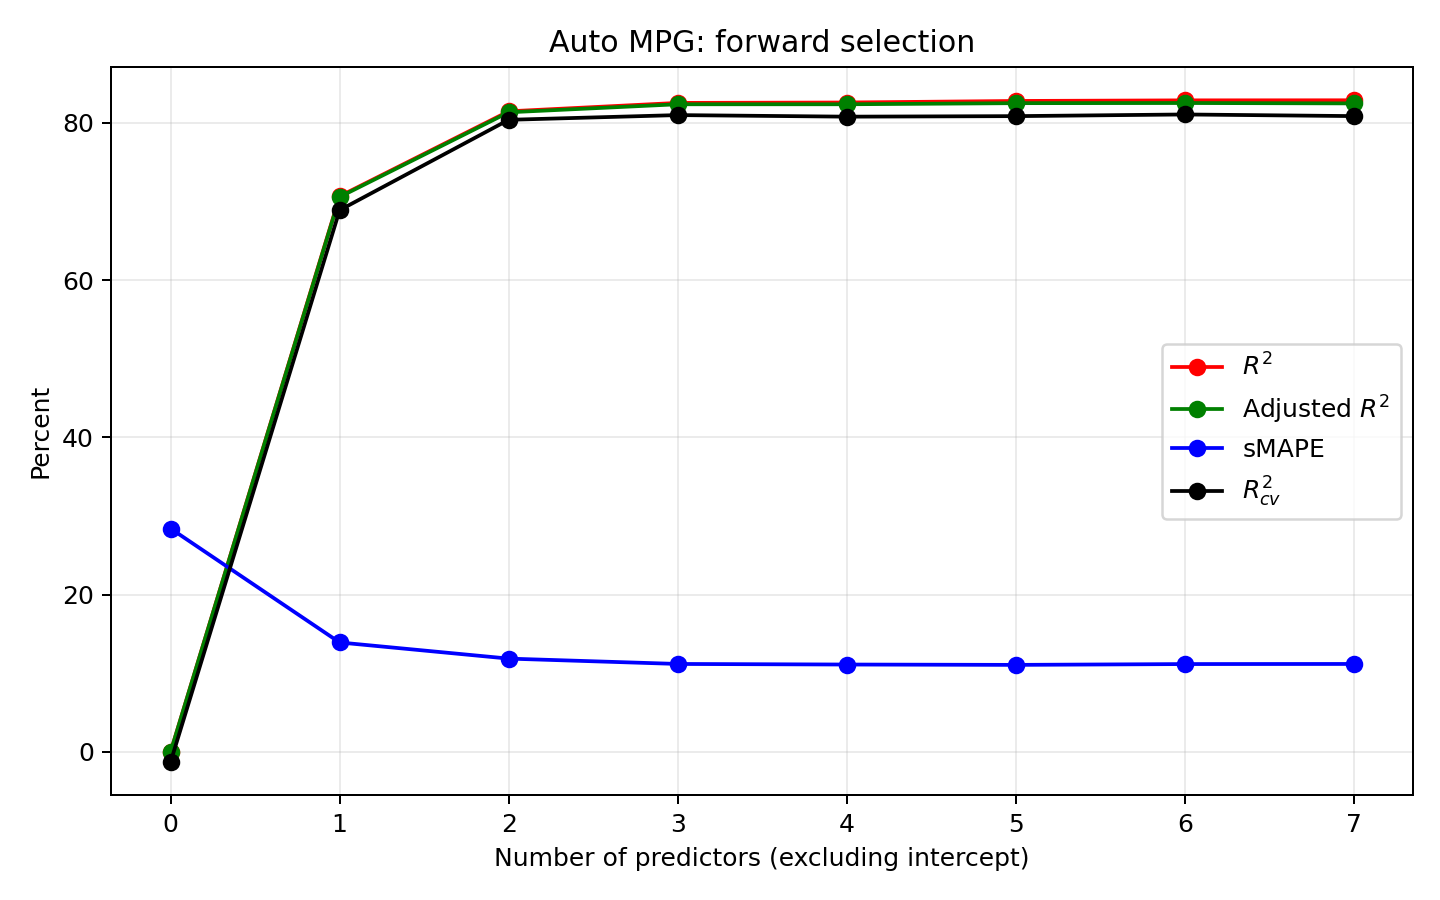
\includegraphics[width=0.6\textwidth]{Forward Selection Images/fs_auto_mpg_r2_vs_n.png}
    \caption{Auto MPG forward selection: $R^2$ (red), adjusted $R^2$ (green), sMAPE (blue), and $R^2_{cv}$ (black) versus the number of predictors.}
    \label{fig:fs-auto-path}
\end{figure}

Adjusted $R^2$ rises sharply with the addition of weight and model year, then flattens. Origin, cylinders, displacement, and horsepower each add only a fraction of a percentage point, and adding acceleration at step 7 decreases adjusted $R^2$ (from 82.52 to 82.47) even though raw $R^2$ still increases slightly. This is the expected behavior of adjusted $R^2$, which penalizes predictors that do not sufficiently improve the fit, and it signals that acceleration is not worth including. sMAPE is also lowest at step 5 rather than improving continuously, which supports the conclusion that the search has saturated.

\vspace{0.3cm}

The maximum adjusted $R^2$ occurs at step 6, so the best model keeps six predictors (weight, model year, origin, cylinders, displacement, and horsepower) plus the intercept and drops only acceleration. Refitting this subset on all 392 observations with \texttt{trainNtest()} gives the coefficients in Table~\ref{tab:fs-auto-coef} and the actual versus predicted plot in Figure~\ref{fig:fs-auto-fit}.

\begin{table}[H]
    \centering
    \caption{Coefficients of the best Auto MPG forward selection model (full-data refit).}
    \label{tab:fs-auto-coef}
    \begin{tabular}{lc}
        \hline
        Variable & Coefficient \\
        \hline
        intercept & $-15.563492$ \\
        weight & $-0.006218$ \\
        model year & 0.747516 \\
        origin & 1.428242 \\
        cylinders & $-0.506685$ \\
        displacement & 0.019269 \\
        horsepower & $-0.023895$ \\
        \hline
    \end{tabular}
\end{table}

\begin{figure}[H]
    \centering
    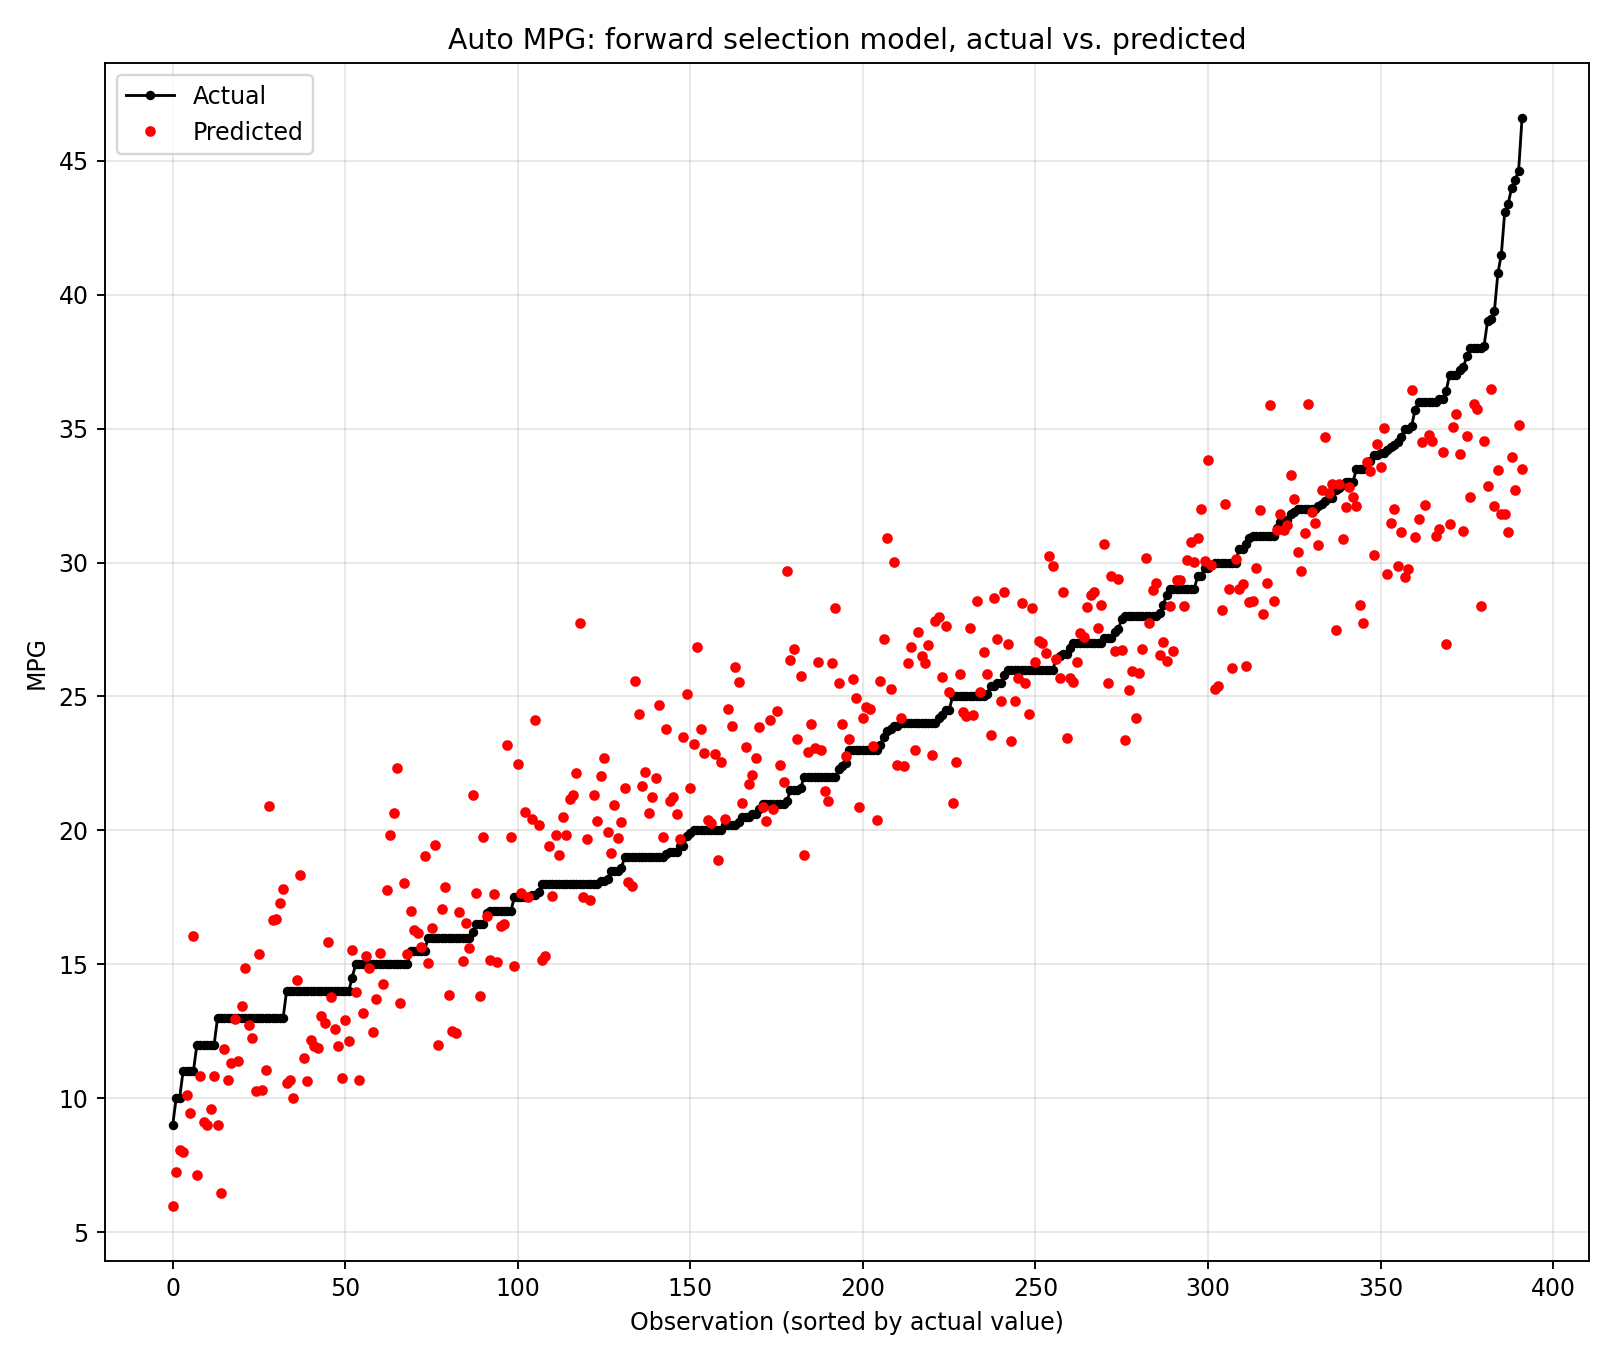
\includegraphics[width=0.6\textwidth]{Forward Selection Images/fs_auto_mpg_actual_vs_pred.png}
    \caption{Actual (black) and predicted (red) MPG for the best Auto MPG forward selection model, with observations sorted by actual value.}
    \label{fig:fs-auto-fit}
\end{figure}

The selected model achieved an $R^2$ of 0.8212, an adjusted $R^2$ of 0.8184, and an RMSE of 3.296 MPG on the full dataset. Its 5-fold cross-validated $R^2_{cv}$ was 0.8106, which evaluates the fixed selected subset across folds; selection was not repeated inside each fold, so this is not a nested-CV estimate of the complete selection procedure. This is a large improvement over the best simple regression (weight alone, $R^2 = 0.6926$), and it is essentially the same fit as the full seven-predictor model from the multiple regression section (adjusted $R^2$ of 0.8182), so dropping acceleration changes the descriptive fit very little. Heavier cars and cars with more cylinders are associated with lower MPG, while later model years are associated with higher MPG, which is consistent with improvements in fuel efficiency over the 1970--1982 sample period. The displacement coefficient is slightly positive even though displacement is negatively correlated with MPG on its own. This is likely because weight, cylinders, and displacement are strongly correlated with one another, so once weight and cylinders are in the model, displacement no longer plays its marginal role.

\subsubsection{Concrete}

Forward selection considered all eight predictors (cement, blast furnace slag, fly ash, water, superplasticizer, coarse aggregate, fine aggregate, and age) for compressive strength. Table~\ref{tab:fs-concrete-path} lists the selection path, and Figure~\ref{fig:fs-concrete-path} plots the metrics against the number of predictors.

\begin{table}[H]
    \centering
    \caption{Forward selection path for Concrete (values in \%). Adjusted $R^2$ peaks at step 8. Adjusted $R^2$ is computed with the training-set size used by \texttt{forwardSelAll} (823 rows).}
    \label{tab:fs-concrete-path}
    \begin{tabular}{clcccc}
        \hline
        Step & Variable added & $R^2$ & Adjusted $R^2$ & sMAPE & $R^2_{cv}$ \\
        \hline
        0 & intercept & $-0.000$ & $0.00$ & 40.080 & $-1.465$ \\
        1 & cement & 24.566 & 24.47 & 36.919 & 22.857 \\
        2 & superplasticizer & 35.429 & 35.27 & 34.587 & 33.061 \\
        3 & age & 48.513 & 48.32 & 30.110 & 46.730 \\
        4 & blast furnace slag & 54.989 & 54.77 & 28.171 & 53.311 \\
        5 & water & 58.501 & 58.25 & 27.518 & 56.647 \\
        6 & fly ash & 61.754 & 61.47 & 26.216 & 59.805 \\
        7 & fine aggregate & 61.785 & 61.46 & 26.162 & 59.789 \\
        8 & coarse aggregate & 61.888 & \textbf{61.51} & 26.070 & 59.749 \\
        \hline
    \end{tabular}
\end{table}

\begin{figure}[H]
    \centering
    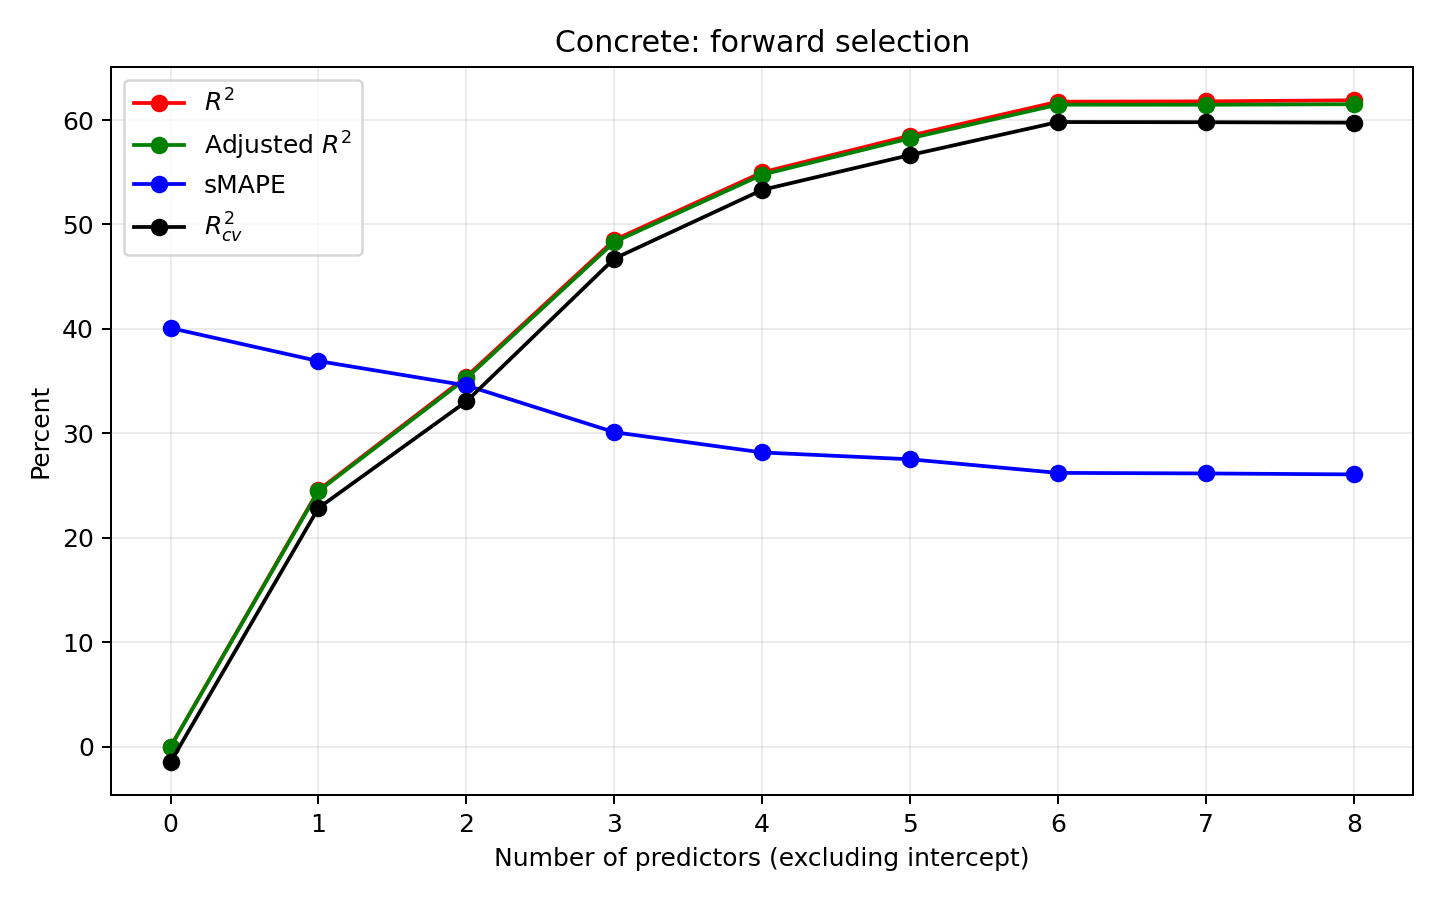
\includegraphics[width=0.6\textwidth]{Forward Selection Images/fs_concrete_r2_vs_n.png}
    \caption{Concrete forward selection: $R^2$ (red), adjusted $R^2$ (green), sMAPE (blue), and $R^2_{cv}$ (black) versus the number of predictors.}
    \label{fig:fs-concrete-path}
\end{figure}

Unlike Auto MPG, adjusted $R^2$ for Concrete keeps increasing through nearly the whole path. The one exception is a tiny dip at step 7 (61.47 to 61.46), and step 8 then reaches the maximum, so the full model narrowly wins. The largest gains come from cement and superplasticizer, the two predictors most correlated with compressive strength, followed by a large jump from age. Blast furnace slag, water, and fly ash then add roughly 6.5, 3.5, and 3.2 points of adjusted $R^2$ respectively, while fine and coarse aggregate together add less than 0.1 points, which appears as the flat tail of the curve in Figure~\ref{fig:fs-concrete-path}. sMAPE drops from 40.1\% for the intercept-only model to about 26\% by step 6 and barely changes afterward.

\vspace{0.3cm}

Because adjusted $R^2$ is highest at step 8, the best model keeps all eight predictors plus the intercept. Table~\ref{tab:fs-concrete-coef} gives the coefficients from the full-data refit, and Figure~\ref{fig:fs-concrete-fit} shows the actual versus predicted values.

\begin{table}[H]
    \centering
    \caption{Coefficients of the best Concrete forward selection model (full-data refit).}
    \label{tab:fs-concrete-coef}
    \begin{tabular}{lc}
        \hline
        Variable & Coefficient \\
        \hline
        intercept & $-23.163756$ \\
        cement & 0.119785 \\
        superplasticizer & 0.290687 \\
        age & 0.114226 \\
        blast furnace slag & 0.103847 \\
        water & $-0.150298$ \\
        fly ash & 0.087943 \\
        fine aggregate & 0.020154 \\
        coarse aggregate & 0.018030 \\
        \hline
    \end{tabular}
\end{table}

\begin{figure}[H]
    \centering
    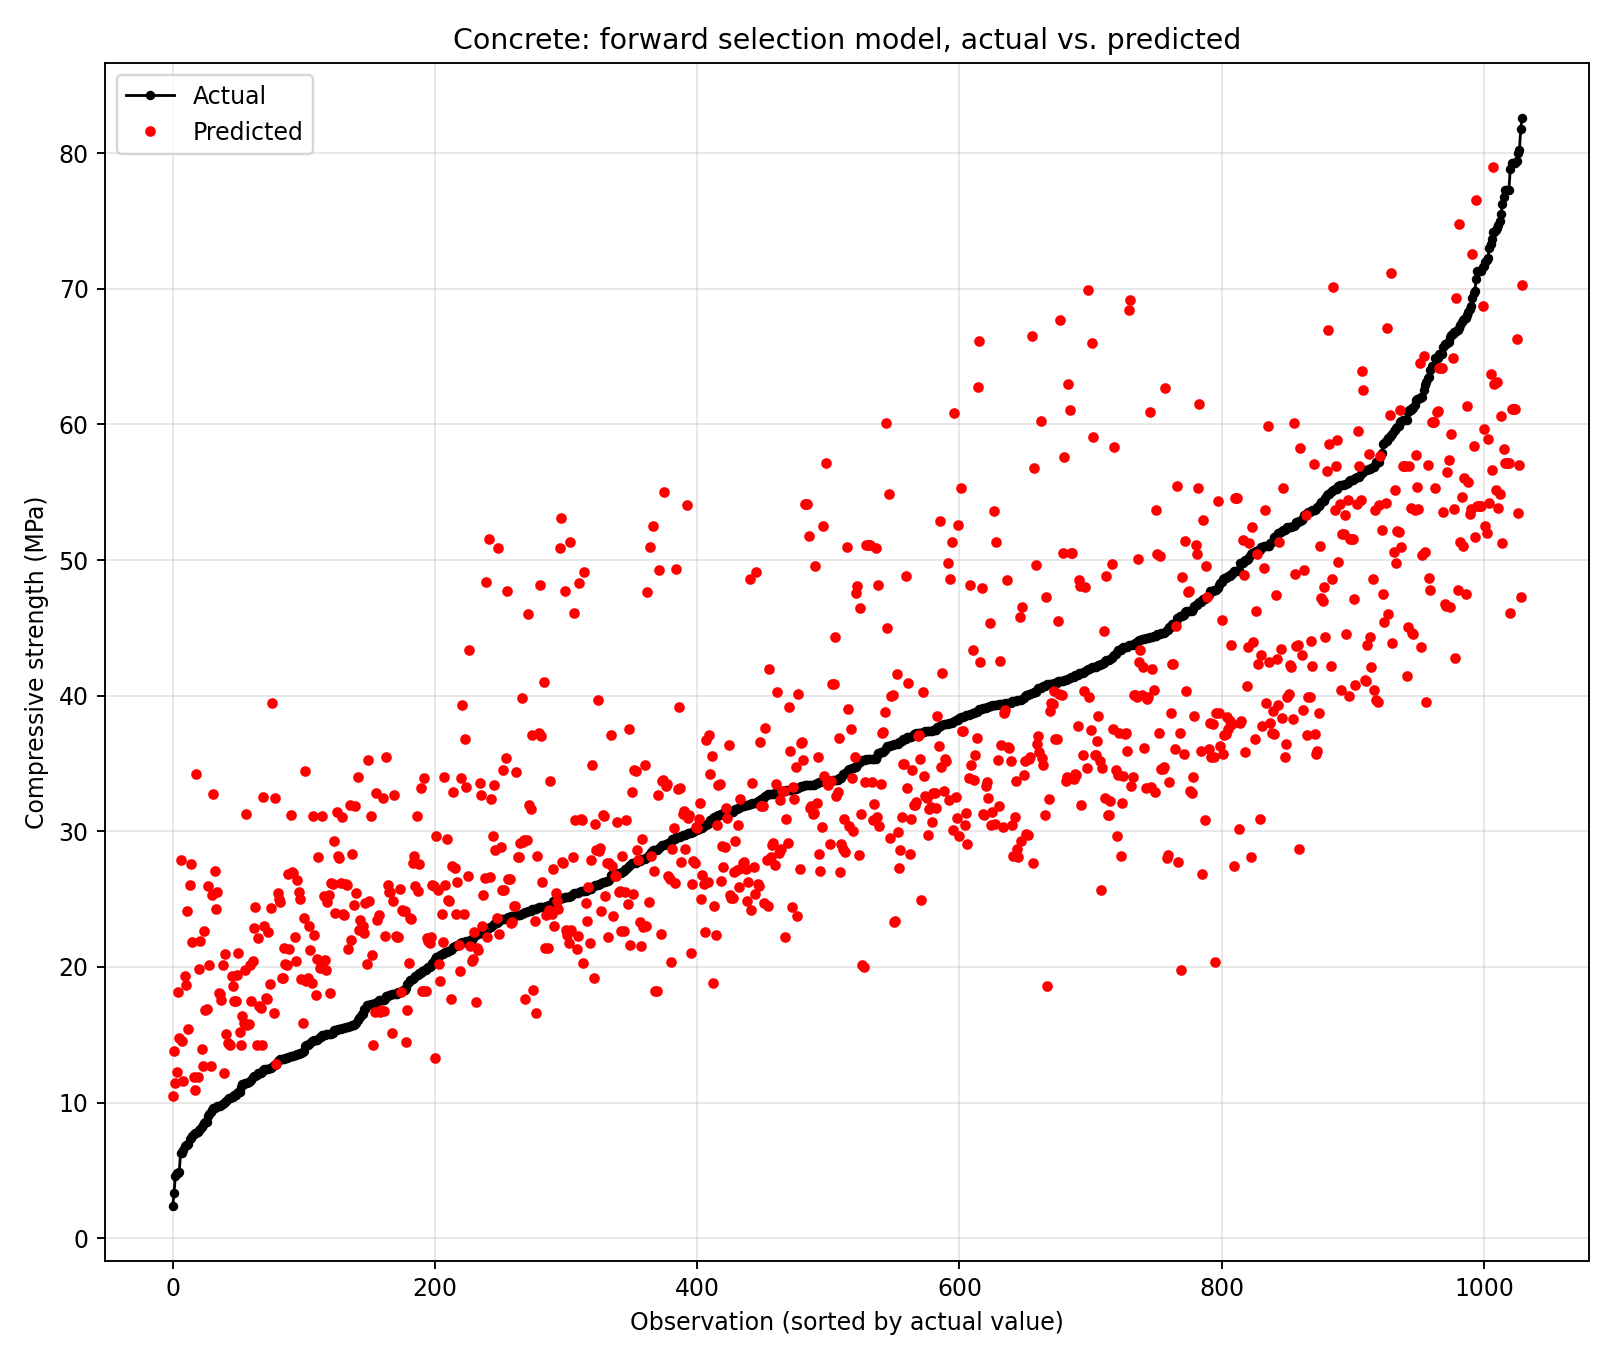
\includegraphics[width=0.6\textwidth]{Forward Selection Images/fs_concrete_actual_vs_pred.png}
    \caption{Actual (black) and predicted (red) compressive strength for the best Concrete forward selection model, with observations sorted by actual value.}
    \label{fig:fs-concrete-fit}
\end{figure}

The selected model achieved an $R^2$ of 0.6155, an adjusted $R^2$ of 0.6125, and an RMSE of 10.354 MPa on the full dataset, with a cross-validated $R^2_{cv}$ of 0.5975. This is a marked improvement over the best simple regression (cement alone, $R^2 = 0.2478$) and matches the full multiple regression model. All coefficients are positive except water, which agrees with domain expectations: a higher water content at fixed cement, meaning a higher water-to-cement ratio, is associated with lower strength. The actual versus predicted plot shows much wider scatter than for Auto MPG, particularly for mid-range strengths, which is consistent with the moderate $R^2$ and suggests that a large share of the variability is not captured by linear terms alone.

\subsection{Summary}

In both datasets, forward selection guided by adjusted $R^2$ chose the same leading predictors as the correlation analysis in the multiple regression section: weight came first for Auto MPG, and cement and superplasticizer came first for Concrete. The two datasets behave differently after that. For Auto MPG, adjusted $R^2$ saturates quickly and declines when acceleration is forced in, so the retained subset contains six of seven predictors even though the path visits all seven. For Concrete, adjusted $R^2$ keeps climbing, however modestly, to the full model, so no variables are excluded. In both cases the selected model performs about as well as the full multiple regression model, and the cross-validated $R^2_{cv}$ (0.8106 and 0.5975) is a little lower than the full-data $R^2$, as expected. This highlights why adjusted $R^2$ is a better selection criterion than raw $R^2$, which never decreases as predictors are added.

\section{Transformed Regression}


Transformed regression keeps the linear model and its efficient least-squares training but applies a transformation $f$ to the response:
\[
f(y) = \mathbf{b}\cdot\mathbf{x} + \epsilon, \qquad \hat{y} = f^{-1}(\mathbf{b}\cdot\mathbf{x}).
\]
It was fitted with ScalaTion's \texttt{TranRegression} class on two of the three datasets, Auto MPG and Concrete, using all available predictors plus an intercept. For each dataset, five models were compared: plain \texttt{Regression} (no transformation) and \texttt{TranRegression} with a log, square-root, reciprocal, and Box-Cox transformation,
\[
f_\lambda(y) = \frac{y^{\lambda}-1}{\lambda}\ (\lambda \neq 0), \qquad f_0(y) = \log y .
\]
The transformed variable is the response only: fuel economy (\texttt{mpg}, in MPG) for Auto MPG and compressive strength (\texttt{compressive\_strength\_mpa}, in MPa) for Concrete. Predictor variables are left untransformed. Box--Cox was selected as the required alternative to Yeo--Johnson; since every observed response is strictly positive, Yeo--Johnson's extension to nonpositive values is not needed. The reciprocal transformation is included as an additional comparison.

Because $\lambda = 1$ is a shift of $y$, the Box-Cox family contains ``no transformation'' as a special case. The Box-Cox parameter was tuned over $\lambda \in \{-1, -0.75, \dots, 2\}$ by 5-fold cross-validation on the training set only. Predictions were mapped back with $f^{-1}$, so the comparison tables report $R^2$, RMSE, and MAE on the \emph{original} response scale. Full-data fits are descriptive; held-out results come from separate models fitted only to the training rows. Both datasets use an 80/20 split generated by Scala's random shuffle with seed 42. For Auto MPG, this reproduces the split used by the existing ScalaTion Ridge and Lasso code. Auto MPG uses 314 training and 78 test rows; Concrete uses 824 training and 206 test rows. The already shuffled training rows are divided into five contiguous folds, and CV RMSE pools squared errors across all validation rows. All observed responses are positive. For $\lambda\ne0$, a valid Box--Cox inverse requires $1+\lambda z>0$, even when an integer inverse power would return a finite number outside this domain. Square-root and positive-response reciprocal models require $z\geq0$ and $z>0$, respectively. Candidates with any invalid or nonfinite validation prediction are excluded. An invalid full-data or test prediction makes that entire model/split score unavailable; rows are never silently discarded.

Auto MPG and Concrete satisfy the requirement to apply transformed regression to two of the three datasets. They provide a useful comparison because the observed benefit is substantial for Auto MPG and small for Concrete. No transformed-regression result is claimed for Airfoil.

The predictions use direct inverse transformation, without a retransformation bias correction. In general, $f^{-1}(E[f(y)\mid x])$ is not $E[y\mid x]$; these fits minimize squared error on the transformed scale, not the original scale. Original-scale validation measures the practical prediction error of this choice. The chosen $\lambda$ minimizes training CV RMSE; the held-out test set is not used for tuning.

\subsection{Auto MPG}

\begin{table}[H]
\centering
\small
\begin{tabular}{lrrr|rrr}
\toprule
 & \multicolumn{3}{c|}{In-sample ($n=392$)} & \multicolumn{3}{c}{Held-out test} \\
Model & $R^2$ & RMSE & MAE & $R^2$ & RMSE & MAE \\
\midrule
Regression (no transform)      & 0.8215 & 3.294 & 2.499 & 0.7835 & 3.528 & 2.631 \\
TranRegression, log            & 0.8562 & 2.956 & 2.102 & 0.8216 & 3.202 & 2.285 \\
TranRegression, sqrt           & 0.8437 & 3.082 & 2.252 & 0.8059 & 3.340 & 2.426 \\
TranRegression, reciprocal     & 0.8490 & 3.029 & 2.137 & 0.8069 & 3.331 & 2.274 \\
TranRegression, Box-Cox $\lambda=-0.5$ & \textbf{0.8612} & \textbf{2.904} & \textbf{2.043} & \textbf{0.8279} & \textbf{3.145} & \textbf{2.216} \\
\bottomrule
\end{tabular}
\caption{Auto MPG: original-scale quality of fit for plain and transformed regression (ScalaTion).}
\label{tab:tran_autompg}
\end{table}

Every transformation improved on plain regression, both in-sample and on the test set. Cross-validation selected $\lambda = -0.5$ (CV RMSE 2.995 versus 3.391 at $\lambda = 1$), and this model reduced test RMSE from 3.528 to 3.145~MPG, a 10.9\% reduction. The selected $\lambda$ lies between the log ($\lambda = 0$) and reciprocal ($\lambda = -1$) transformations. The reciprocal alternative models fuel consumption (gallons per mile, $1/\text{MPG}$) directly; its improvement over plain regression supports examining nearby powers.

Figure~\ref{fig:tran_autompg} compares full-data fits and residuals. The Box--Cox model improves the fit, but these plots are descriptive and do not replace the held-out evaluation. On the transformed scale, the selected full-data model has $R^2=0.890$. Model year ($t=15.9$) and weight ($t=-10.7$) have the largest absolute $t$ statistics among its predictors. Acceleration has $p=0.23$. These are conventional OLS statistics conditional on the selected transformation, without adjustment for choosing $\lambda$ from the data; they are descriptive rather than confirmatory. Coefficients and their standard errors are computed on the transformed scale and are not in MPG units. Origin is treated as a numeric predictor, matching the existing regression setup.

\begin{figure}[H]
\centering
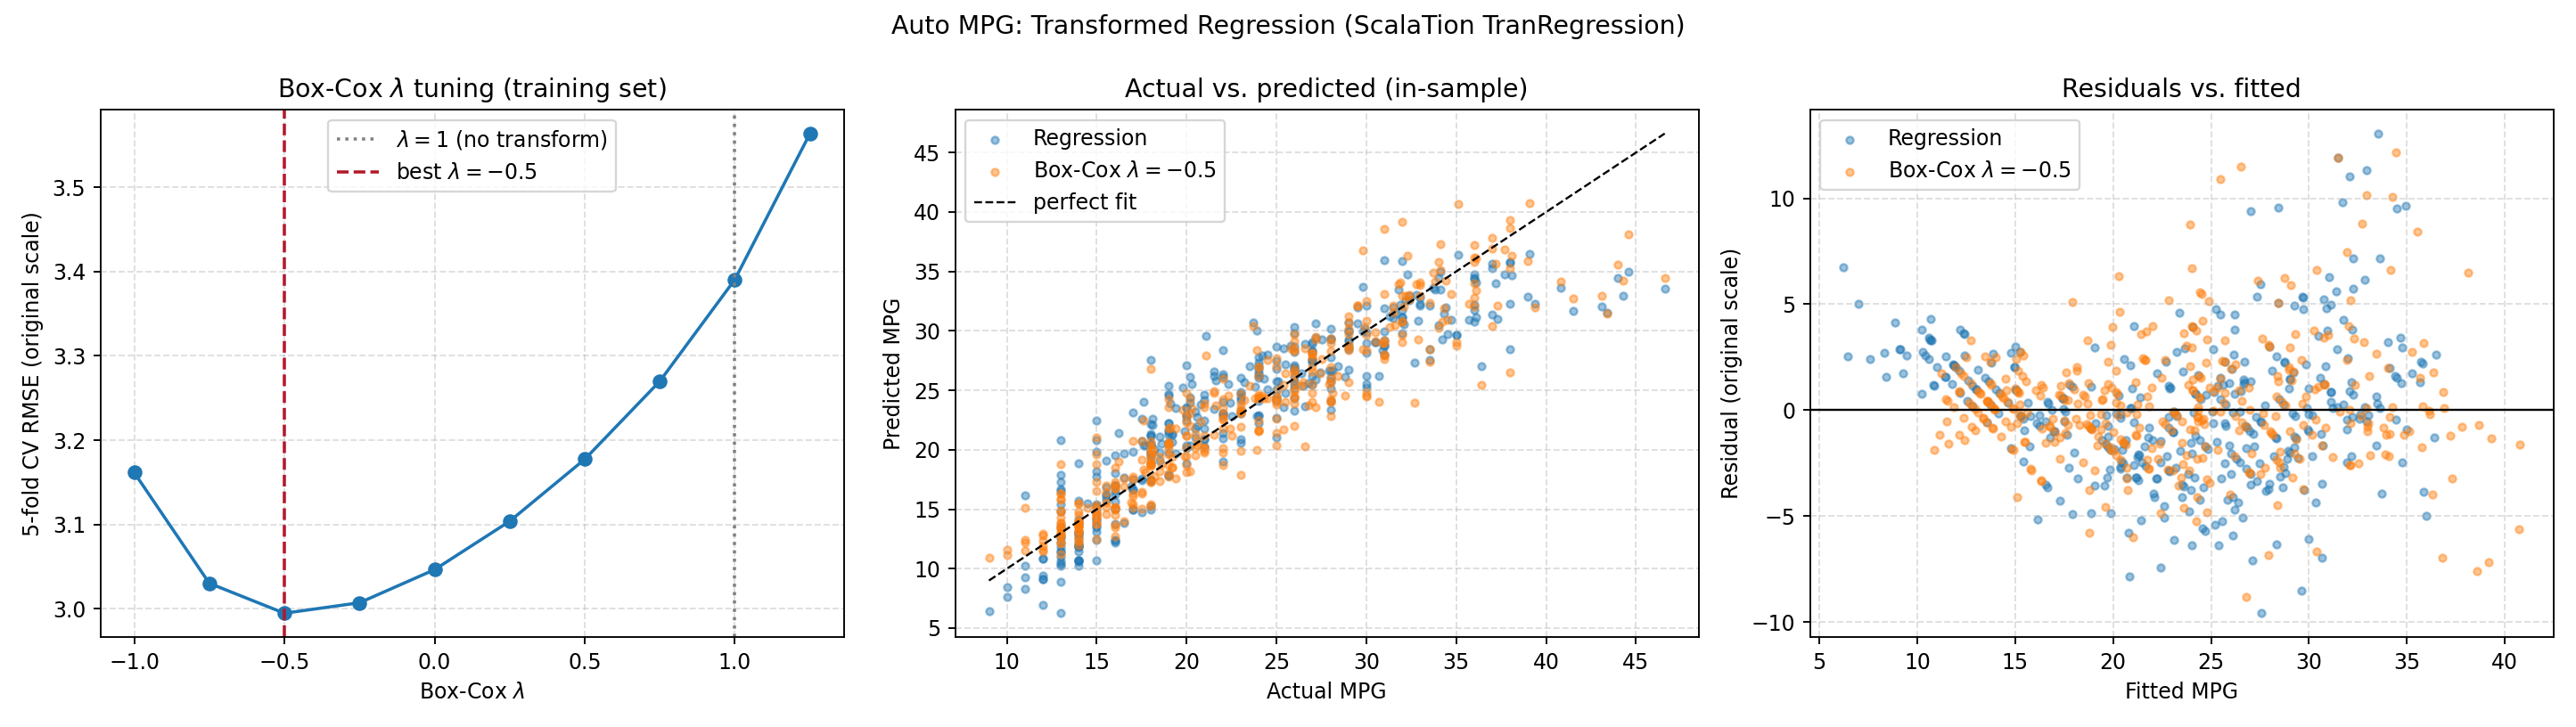
\includegraphics[width=\textwidth]{Transformed Regression Images/auto_mpg_transformed_regression.png}
\caption{Auto MPG: Box-Cox $\lambda$ tuning curve (left), actual vs.\ predicted MPG (center), and residuals vs.\ fitted values (right) for plain regression and the Box-Cox $\lambda=-0.5$ model.}
\label{fig:tran_autompg}
\end{figure}

\subsection{Concrete}

\begin{table}[H]
\centering
\small
\begin{tabular}{lrrr|rrr}
\toprule
 & \multicolumn{3}{c|}{In-sample ($n=1030$)} & \multicolumn{3}{c}{Held-out test} \\
Model & $R^2$ & RMSE & MAE & $R^2$ & RMSE & MAE \\
\midrule
Regression (no transform)      & 0.6155 & 10.354 & 8.215 & 0.5957 & 10.311 & 8.125 \\
TranRegression, log            & 0.4559 & 12.317 & 9.442 & 0.4740 & 11.761 & 9.305 \\
TranRegression, sqrt           & 0.5800 & 10.822 & 8.637 & 0.5582 & 10.779 & 8.571 \\
TranRegression, reciprocal     & --- & --- & --- & --- & --- & --- \\
TranRegression, Box-Cox $\lambda=1.25$ & \textbf{0.6218} & \textbf{10.269} & \textbf{8.074} & \textbf{0.6055} & \textbf{10.185} & \textbf{7.970} \\
\bottomrule
\end{tabular}
\caption{Concrete: original-scale quality of fit. Reciprocal scores are unavailable because the positive-response inverse domain fails for 21 of 1,030 full-data predictions and 1 of 206 test predictions.}
\label{tab:tran_concrete}
\end{table}

Concrete benefits much less from response transformation. Log and square-root transformations increased prediction error relative to plain regression: log reduced test $R^2$ from 0.596 to 0.474, and square root reduced it to 0.558. The reciprocal transformation failed badly. The model on $1/y$ produces some nonpositive fitted values, outside the inverse domain for positive strengths. Near-zero positive values can also produce very large predictions. This makes the reciprocal model unsuitable here. Cross-validation chose $\lambda = 1.25$, slightly \emph{above} 1, which expands rather than compresses the response. The resulting gain is marginal: test RMSE fell only from 10.311 to 10.185~MPa (1.2\%). The valid portion of the CV curve in Figure~\ref{fig:tran_concrete} is nearly flat between $\lambda=0.75$ and $1.5$ (CV RMSE 10.43 at the optimum versus 10.51 with no transformation), so the data provide little evidence for any response transformation.

These results show that transforming only the response offers limited benefit for this linear predictor specification. They do not establish the source of any remaining nonlinearity. Transforming predictors or adding interactions could be investigated separately through symbolic regression. The small improvement on one held-out split is not evidence of a statistically significant gain.

\begin{figure}[H]
\centering
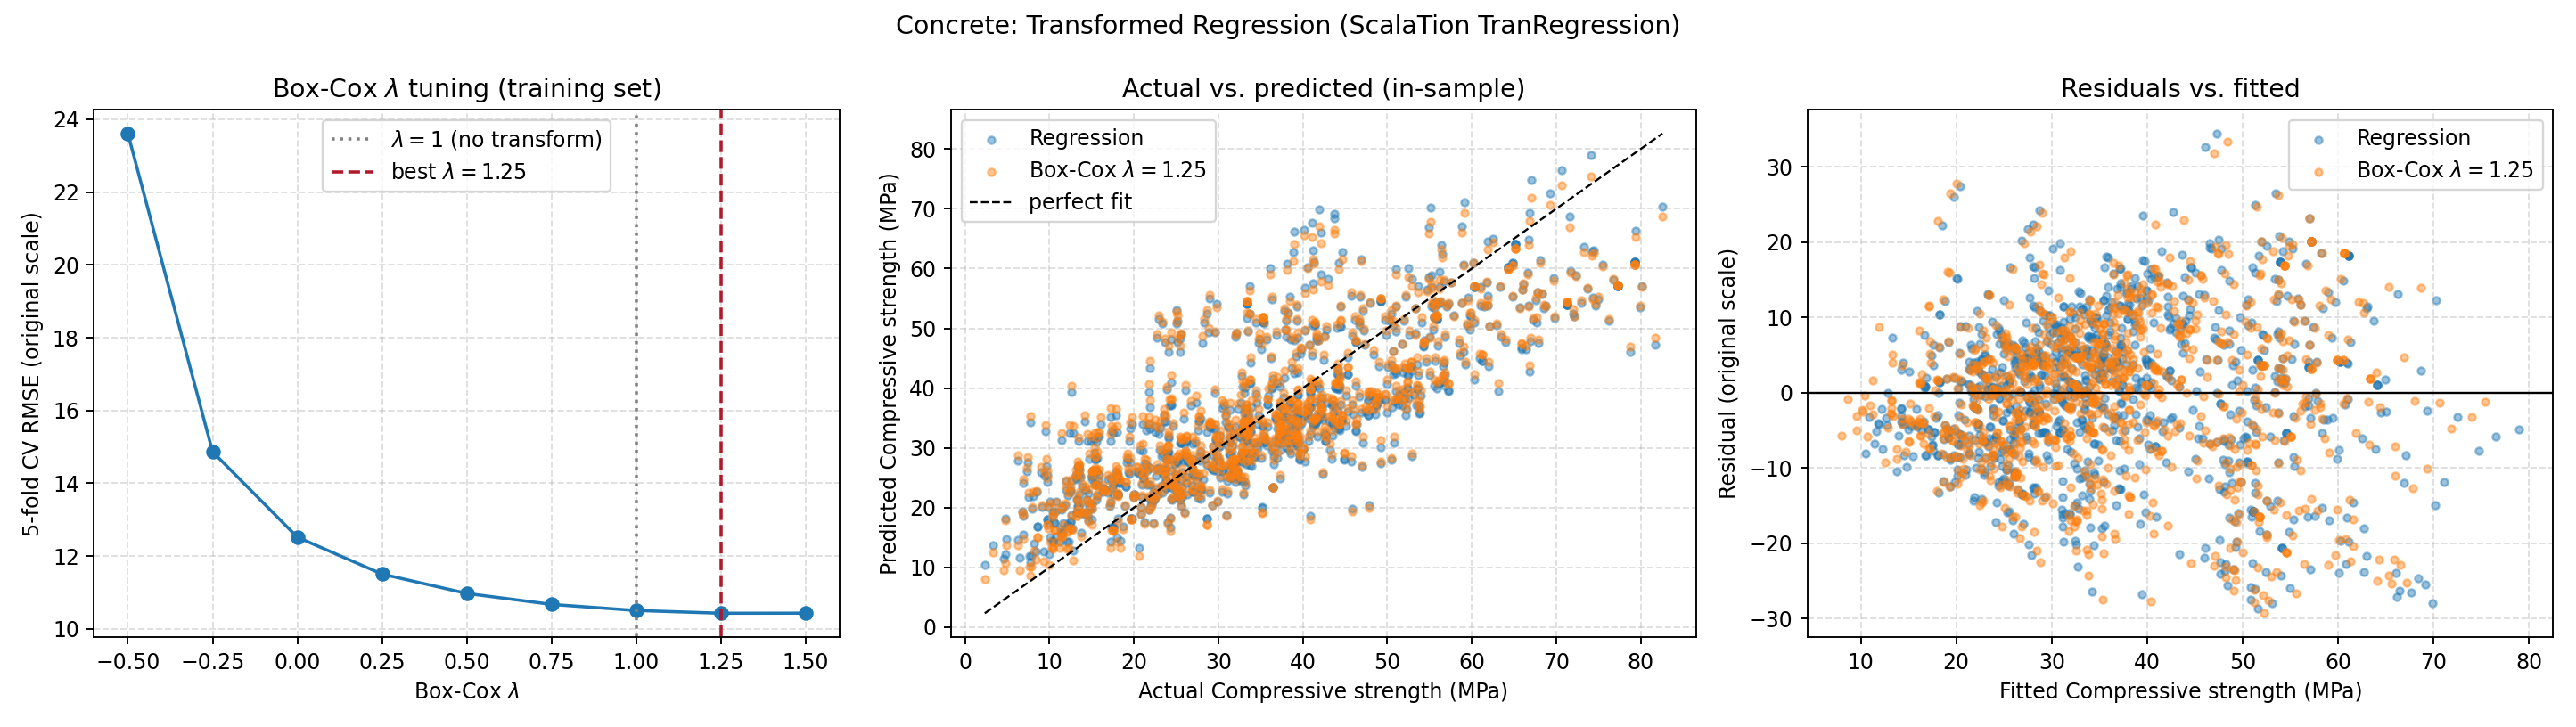
\includegraphics[width=\textwidth]{Transformed Regression Images/concrete_transformed_regression.png}
\caption{Concrete: Box-Cox $\lambda$ tuning curve (left; invalid candidates omitted), actual vs.\ predicted strength (center), and residuals vs.\ fitted values (right) for plain regression and the Box-Cox $\lambda=1.25$ model.}
\label{fig:tran_concrete}
\end{figure}

\subsection{Summary}

For Auto MPG, training CV selected Box--Cox $\lambda=-0.5$, and test RMSE fell by 10.9\% relative to plain regression. For Concrete, $\lambda=1.25$ reduced test RMSE by only 1.2\%; log and square-root transformations worsened test error, and the reciprocal model produced invalid predictions. These conclusions apply to the tested models and this fixed split, not to all possible ScalaTion or symbolic-regression models. A response transformation should be chosen using validation in the units of the prediction task.

\section{Symbolic Regression}

Symbolic regression differs from traditional linear regression because it
searches not only for model coefficients, but also for the mathematical
structure relating the predictors to the response. Instead of assuming a
predefined functional form, symbolic regression searches over combinations
of mathematical operators and variables to identify equations that balance
predictive accuracy and expression complexity.

Two symbolic regression implementations were used in this project:
ScalaTion and PySR. ScalaTion constructs transformed candidate features and
applies feature selection, while PySR uses an evolutionary search procedure
to discover mathematical expressions directly. The three datasets analyzed
were Auto MPG, Concrete Compressive Strength, and Airfoil Self-Noise.

\subsection{ScalaTion}

ScalaTion's \texttt{SymbolicRegression} builds candidate basis functions, and forward selection retains a subset for a linear combination of nonlinear terms. Predictor names are read from the CSV headers, so cylinders and displacement are identified in the repository's actual order. Each dataset is shuffled with Scala seed 42 and split \emph{before} any fitting or selection. The training/test sizes are 314/78 for Auto MPG, 824/206 for Concrete, and 1203/300 for Airfoil. Feature construction uses predefined operators; means, scales, numerical-rank screening, and feature selection use training rows only. The test rows are reserved until the final selected model is fitted.

Auto MPG uses powers $-2,-1,1/2,2$; Concrete uses $1,1/2,2$; Airfoil uses $1,1/2,2$, $\log(1+x)$, two-way and three-way products of distinct predictors, and $c/(f d^{3/2})$. Here $c$, $f$, and $d$ denote chord length, frequency, and suction displacement thickness. Powers and operator sets are fixed before evaluation. All transformations are finite for the observed predictors.

Each nonconstant basis function is centered and scaled using its training mean and population standard deviation. In candidate order, two-pass Gram--Schmidt screening rejects columns whose residual norm is at most $10^{-6}$ of their original standardized norm. This removes numerically redundant functions using only the training design. There are 28/24/41 initial nonconstant candidates for Auto MPG/Concrete/Airfoil and 26/24/40 after screening. Forward selection minimizes the library's training $\mathrm{sMAPE}_{IC}$ criterion over the complete selection path. The final subset is refitted by QR least squares on all outer training rows; test predictions use those same training scaling constants. No random validation calls or test responses enter selection.

These results describe predictive performance on one fixed split. Selecting correlated nonlinear features does not establish confirmatory effects or causal relationships.

\begin{table}[H]
\centering\small
\caption{ScalaTion symbolic regression: training fit and untouched test-set performance. RMSE/MAE use each response's original units.}
\label{tab:scalation-symbolic-results}
\begin{tabular}{lrrrrrrr}
\toprule
Dataset & $n_{tr}$ & $n_{te}$ & Terms & Train $R^2$ & Test $R^2$ & RMSE & MAE \\
\midrule
Auto MPG & 314 & 78 & 17 & 0.8918 & 0.8650 & 2.7853 & 2.0858 \\
Concrete & 824 & 206 & 18 & 0.8556 & 0.8237 & 6.8098 & 5.0507 \\
Airfoil & 1203 & 300 & 22 & 0.7071 & 0.7113 & 3.9985 & 3.0940 \\
\bottomrule
\end{tabular}
\end{table}

\begin{table}[H]
\centering\small
\caption{Linear baseline and symbolic regression on identical Scala test rows. Positive reductions indicate lower symbolic RMSE.}
\label{tab:symbolic-baseline}
\begin{tabular}{lrrrr}
\toprule
Dataset & Linear $R^2$ & Linear RMSE & Symbolic RMSE & RMSE reduction (\%) \\
\midrule
Auto MPG & 0.7835 & 3.5276 & 2.7853 & 21.0 \\
Concrete & 0.5957 & 10.3108 & 6.8098 & 34.0 \\
Airfoil & 0.5377 & 5.0598 & 3.9985 & 21.0 \\
\bottomrule
\end{tabular}
\end{table}

\subsubsection{Auto MPG}

The model retained 17 nonconstant terms plus an intercept. Test $R^2=0.8650$, RMSE $=2.7853$~MPG, and MAE $=2.0858$~MPG. Against linear regression on the same training/test rows, RMSE falls from 3.5276 to 2.7853~MPG (21.0\%). The selected expression includes inverse weight, nonlinear model year, inverse displacement and horsepower, acceleration, origin, and cylinder terms. Individual signs belong to a joint nonlinear combination and should not be interpreted as isolated effects. Numeric origin coding follows the other ScalaTion models.

$C,D,H,W,A,Y,O$ are cylinders, displacement, horsepower, weight, acceleration, model year (70--82), and numeric origin, respectively.
The complete fitted expression is
\begin{equation}
\widehat{y}= 23.41656051 + \sum_{j=1}^{17} b_j\frac{\phi_j-\mu_j}{s_j}.
\end{equation}
The following table specifies \emph{every} term and its fitted coefficient and training scaling constants. Values are rounded to 11 significant digits; full double-precision constants and predictions are exported in the dataset-specific \texttt{project2/results/symbolic/} CSVs. The intercept above is not centered or scaled.

{\scriptsize\setlength{\tabcolsep}{3pt}
\begin{longtable}{rlrrr}
\caption{Complete Auto MPG ScalaTion symbolic expression parameters.}\label{tab:auto-mpg-symbolic-complete}\\
\toprule
$j$ & $\phi_j$ & $b_j$ & $\mu_j$ & $s_j$ \\
\midrule\endfirsthead
\toprule
$j$ & $\phi_j$ & $b_j$ & $\mu_j$ & $s_j$ \\
\midrule\endhead
1 & $W^{-1}$ & $1.8615882098$ & $0.00036088109269$ & $0.00010023526341$ \\
2 & $Y^{2}$ & $29.797474083$ & $5781.1050955$ & $555.03854096$ \\
3 & $\sqrt{Y}$ & $-27.062913016$ & $8.7121722882$ & $0.20955641849$ \\
4 & $D^{-1}$ & $2.2799083543$ & $0.0066972548638$ & $0.0032418450901$ \\
5 & $H^{-1}$ & $5.4453586983$ & $0.010731868546$ & $0.0035451860794$ \\
6 & $\sqrt{A}$ & $-10.833743774$ & $3.9275763597$ & $0.35007368107$ \\
7 & $H^{-2}$ & $-2.8720099973$ & $0.00012774134683$ & $8.2206002648\times10^{-5}$ \\
8 & $D^{2}$ & $0.44763104365$ & $50103.752389$ & $50732.708911$ \\
9 & $O^{-1}$ & $-2.4951861577$ & $0.78503184713$ & $0.2872354299$ \\
10 & $W^{2}$ & $-0.002618093047$ & $9773975.3185$ & $5631807.4713$ \\
11 & $A^{2}$ & $6.2719398213$ & $249.35197452$ & $88.977326479$ \\
12 & $A^{-1}$ & $-3.7782361382$ & $0.066444714752$ & $0.01250025077$ \\
13 & $O^{-2}$ & $2.1327499778$ & $0.69877919321$ & $0.39846216897$ \\
14 & $C^{-1}$ & $-211.39430164$ & $0.19816878981$ & $0.055715123421$ \\
15 & $C^{2}$ & $86.96592285$ & $33.439490446$ & $20.413039912$ \\
16 & $\sqrt{C}$ & $-220.70956558$ & $2.3225501851$ & $0.3578458204$ \\
17 & $C^{-2}$ & $77.087687267$ & $0.042375044232$ & $0.021491373332$ \\
\bottomrule\end{longtable}}

\subsubsection{Concrete}

The model retained 18 nonconstant terms plus an intercept. Test $R^2=0.8237$, RMSE $=6.8098$~MPa, and MAE $=5.0507$~MPa. Against linear regression on the same training/test rows, RMSE falls from 10.3108 to 6.8098~MPa (34.0\%). The selected expression includes square-root age, linear age, material powers, and square-root material terms. The opposing age functions allow curvature in the fitted response. Terms involving water and superplasticizer occur together with correlated material variables, so coefficient signs alone do not determine monotone or causal effects.

$C,S,F,W,P,G,Q,A$ are cement, slag, fly ash, water, superplasticizer, coarse aggregate, fine aggregate, and age, respectively.
The complete fitted expression is
\begin{equation}
\widehat{y}= 35.656915953 + \sum_{j=1}^{18} b_j\frac{\phi_j-\mu_j}{s_j}.
\end{equation}
The following table specifies \emph{every} term and its fitted coefficient and training scaling constants. Values are rounded to 11 significant digits; full double-precision constants and predictions are exported in the dataset-specific \texttt{project2/results/symbolic/} CSVs. The intercept above is not centered or scaled.

{\scriptsize\setlength{\tabcolsep}{3pt}
\begin{longtable}{rlrrr}
\caption{Complete Concrete ScalaTion symbolic expression parameters.}\label{tab:concrete-symbolic-complete}\\
\toprule
$j$ & $\phi_j$ & $b_j$ & $\mu_j$ & $s_j$ \\
\midrule\endfirsthead
\toprule
$j$ & $\phi_j$ & $b_j$ & $\mu_j$ & $s_j$ \\
\midrule\endhead
1 & $\sqrt{A}$ & $23.656155389$ & $5.7254280183$ & $3.5375665251$ \\
2 & $P$ & $-12.67585707$ & $6.196717233$ & $6.0055418546$ \\
3 & $C^{2}$ & $-4.0693818011$ & $89457.152566$ & $66553.724173$ \\
4 & $A$ & $-15.943274124$ & $45.294902913$ & $64.080173336$ \\
5 & $S^{2}$ & $-5.80934771$ & $13067.958839$ & $19733.387683$ \\
6 & $P^{2}$ & $2.2705664907$ & $74.465837433$ & $121.70369017$ \\
7 & $\sqrt{W}$ & $498.93892269$ & $13.450751397$ & $0.79442410832$ \\
8 & $W^{2}$ & $264.52288688$ & $33416.792537$ & $7814.2275531$ \\
9 & $G^{2}$ & $-75.418638832$ & $955887.37625$ & $151035.31552$ \\
10 & $W$ & $-766.53178093$ & $181.55382282$ & $21.330774894$ \\
11 & $G$ & $221.83800242$ & $974.62109223$ & $77.466785271$ \\
12 & $\sqrt{G}$ & $-145.92291111$ & $31.194126992$ & $1.2439989626$ \\
13 & $F^{2}$ & $2.5587841018$ & $7177.1080962$ & $9530.0833989$ \\
14 & $\sqrt{P}$ & $11.315055059$ & $1.9281674319$ & $1.5744483439$ \\
15 & $\sqrt{S}$ & $-4.8415549755$ & $6.1801313222$ & $6.0860142189$ \\
16 & $C$ & $16.211006443$ & $279.63561893$ & $106.11820386$ \\
17 & $S$ & $17.980109105$ & $75.233592233$ & $86.068957463$ \\
18 & $\sqrt{Q}$ & $1.1268903315$ & $27.733307052$ & $1.460479483$ \\
\bottomrule\end{longtable}}

\subsubsection{Airfoil}

The model retained 22 nonconstant terms plus an intercept. Test $R^2=0.7113$, RMSE $=3.9985$~dB, and MAE $=3.0940$~dB. Against linear regression on the same training/test rows, RMSE falls from 5.0598 to 3.9985~dB (21.0\%). The selected expression combines frequency, chord length, angle of attack, velocity, and displacement thickness through powers and interaction terms. The custom function is explicitly $c/(f d^{3/2})$. Training-only screening removes a redundant velocity-squared term. The $d$ and $\log(1+d)$ terms have large opposing standardized coefficients because their basis functions are nearly collinear, so their contributions must be read together. Individual coefficients remain sensitive to this correlation.

$f,a,c,v,d$ are frequency (Hz), attack angle (degrees), chord length (m), free-stream velocity (m/s), and suction displacement thickness (m), respectively.
The complete fitted expression is
\begin{equation}
\widehat{y}= 124.98748878 + \sum_{j=1}^{22} b_j\frac{\phi_j-\mu_j}{s_j}.
\end{equation}
The following table specifies \emph{every} term and its fitted coefficient and training scaling constants. Values are rounded to 11 significant digits; full double-precision constants and predictions are exported in the dataset-specific \texttt{project2/results/symbolic/} CSVs. The intercept above is not centered or scaled.

{\scriptsize\setlength{\tabcolsep}{3pt}
\begin{longtable}{rlrrr}
\caption{Complete Airfoil ScalaTion symbolic expression parameters.}\label{tab:airfoil-symbolic-complete}\\
\toprule
$j$ & $\phi_j$ & $b_j$ & $\mu_j$ & $s_j$ \\
\midrule\endfirsthead
\toprule
$j$ & $\phi_j$ & $b_j$ & $\mu_j$ & $s_j$ \\
\midrule\endhead
1 & $d\,c\,f$ & $2.0907331538$ & $2.5583964616$ & $4.3923585896$ \\
2 & $c\,f$ & $-6.3563869786$ & $387.41693101$ & $593.00017373$ \\
3 & $\sqrt{v}$ & $2.63246161$ & $7.0477528943$ & $1.0899688109$ \\
4 & $a^{2}$ & $-1.5976476721$ & $77.848246052$ & $109.54757171$ \\
5 & $c/(f d^{3/2})$ & $-1.8476031911$ & $0.55386125824$ & $0.8793875252$ \\
6 & $c\,a\,f$ & $-2.5420196669$ & $1418.358518$ & $2110.3893069$ \\
7 & $v\,c\,f$ & $5.1768231317$ & $20800.60363$ & $36734.349383$ \\
8 & $d^{2}$ & $144.07756335$ & $0.0002766722994$ & $0.00059945257934$ \\
9 & $d\,f$ & $-7.5183251247$ & $21.240659688$ & $35.407511328$ \\
10 & $d\,a\,f$ & $4.7023305598$ & $231.15085714$ & $523.0025419$ \\
11 & $v\,c$ & $-4.0300029837$ & $6.9692954946$ & $5.418806216$ \\
12 & $v\,f$ & $-3.644800794$ & $152817.85869$ & $194136.65947$ \\
13 & $v\,c\,a$ & $4.2722395003$ & $32.951027493$ & $30.827999053$ \\
14 & $f^{2}$ & $1.391969626$ & $18232037.032$ & $43553709.121$ \\
15 & $c^{2}$ & $1.8939173576$ & $0.027583673682$ & $0.030617990612$ \\
16 & $c\,a$ & $-2.0522278615$ & $0.63581077307$ & $0.5345085506$ \\
17 & $v\,a$ & $-3.7240894811$ & $342.42382377$ & $340.70206773$ \\
18 & $v\,a\,f$ & $1.6424787077$ & $760339.98674$ & $1213676.2184$ \\
19 & $d$ & $-6662.8265773$ & $0.010641921767$ & $0.012783653644$ \\
20 & $d\,c\,a$ & $-3.5575207366$ & $0.01125908998$ & $0.020087724236$ \\
21 & $\sqrt{d}$ & $-7.6438418281$ & $0.088161660887$ & $0.053567185076$ \\
22 & $\log(1+d)$ & $6536.7249606$ & $0.010506878897$ & $0.012508642097$ \\
\bottomrule\end{longtable}}

\begin{figure}[H]
\centering
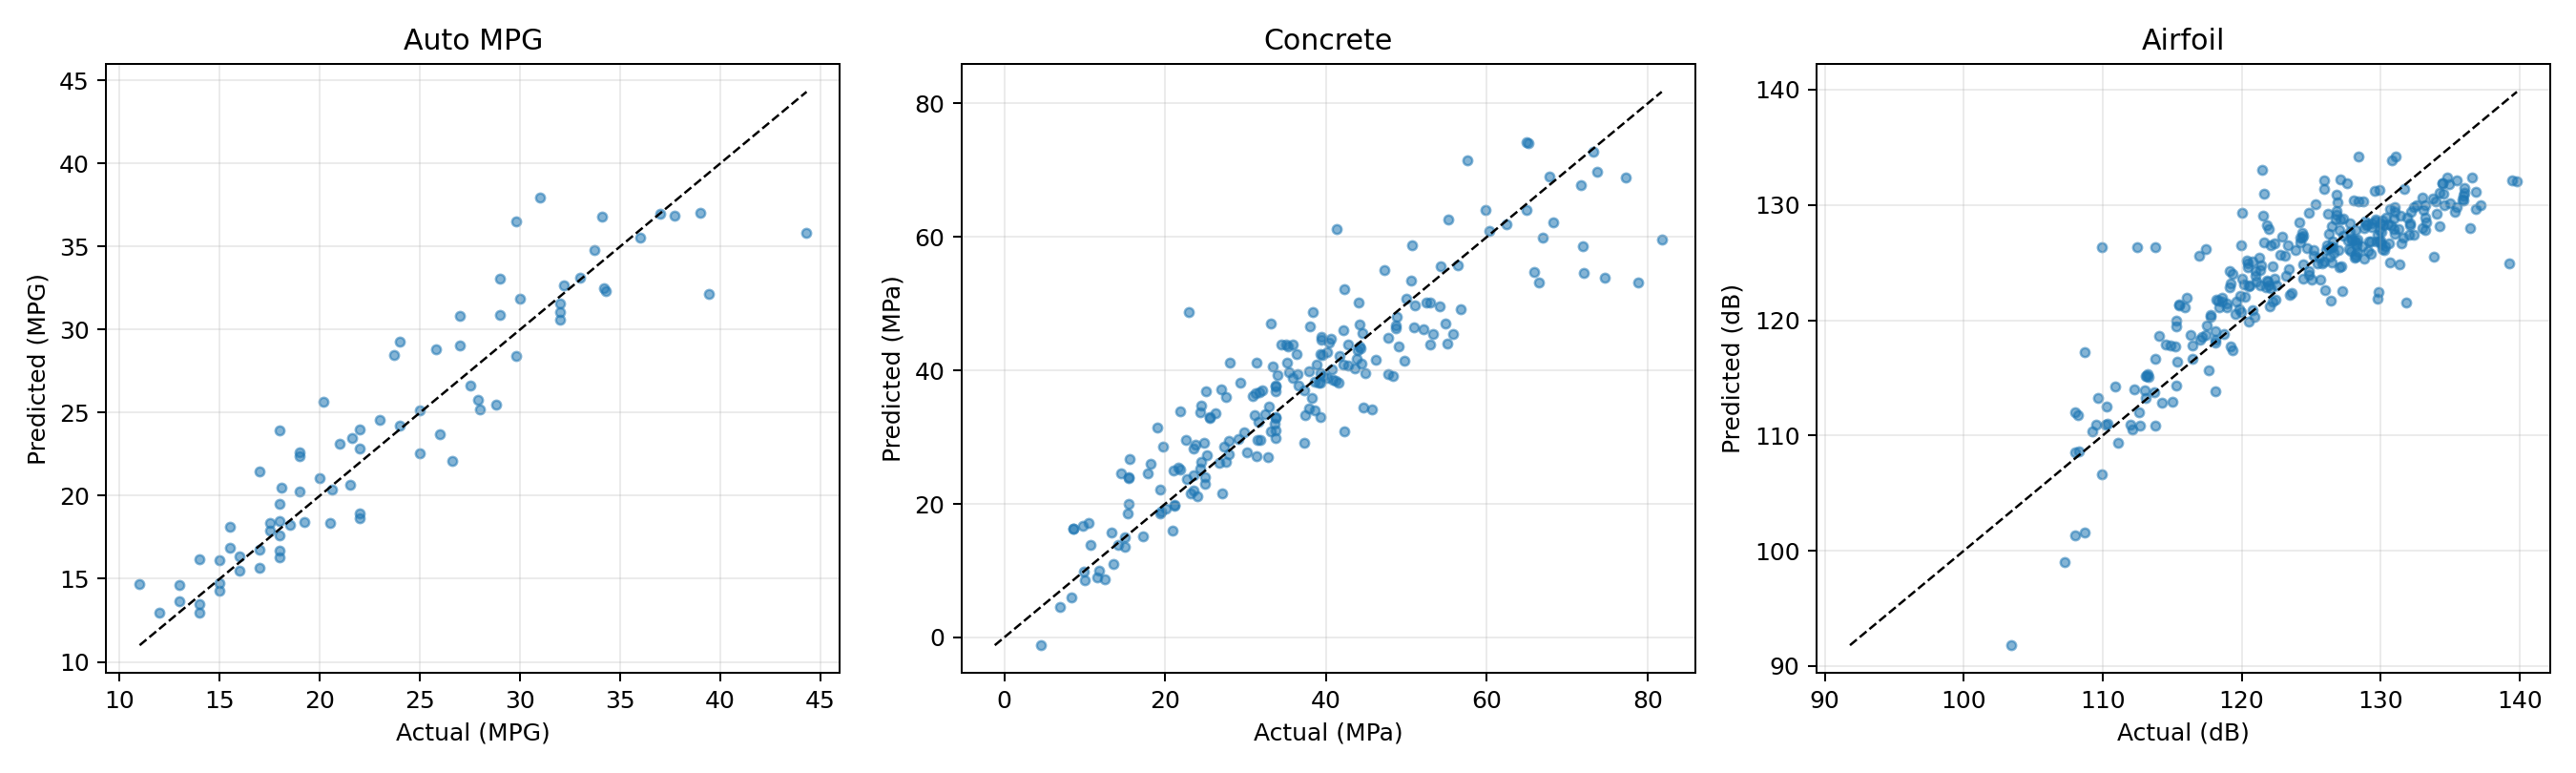
\includegraphics[width=\textwidth]{Symbolic Regression Images/scalation_symbolic_test_predictions.png}
\caption{ScalaTion symbolic predictions on test rows reserved before fitting and selection. The diagonal represents perfect prediction.}
\label{fig:scalation-symbolic-test}
\end{figure}

\subsection{PySR}

PySR was also used to perform symbolic regression on all three datasets.
Each dataset was divided into training and testing sets using an 80/20 split
with \texttt{random\_state=42}. PySR searches for mathematical expressions
through an evolutionary procedure and evaluates candidate expressions based
on predictive loss and expression complexity.

The reported PySR scores are from the saved search outputs. Auto MPG used serial deterministic search with seed 42; Concrete and Airfoil used multithreading, so their search trajectories are not guaranteed repeatable from a seed alone.

The operator set included the binary operators

\[
+, \quad -, \quad \times, \quad /
\]

and nonlinear unary transformations including square root and squared terms.
For the Concrete and Airfoil datasets, logarithmic transformations were also
included.

\subsubsection{Auto MPG}

The Auto MPG dataset contained 392 observations and seven predictors:
displacement, cylinders, horsepower, weight, acceleration, model year, and
origin. The data were divided into 313 training observations and 79 testing
observations.

PySR was run for 150 iterations with the operators
\texttt{+}, \texttt{-}, \texttt{*}, and \texttt{/}, together with the
\texttt{square} and \texttt{sqrt} unary operators. Expression complexity was
limited using \texttt{maxsize=30}, and model selection was performed using
the \texttt{best} criterion.

The selected equation was

\begin{equation}
\widehat{\mathrm{MPG}}
=
\frac{2149.9915(\mathrm{model\_year}-46.281776)}
{\mathrm{weight}}.
\end{equation}

This expression indicates that predicted fuel economy increases with model
year and decreases with vehicle weight. Despite the availability of seven
predictors, PySR selected a compact equation involving only model year and
weight.

On the held-out test set, the model achieved

\[
\mathrm{MSE}=7.5596,
\qquad
\mathrm{RMSE}=2.7495,
\]

\[
\mathrm{MAE}=2.0550,
\qquad
R^2=0.8519.
\]

\begin{figure}[H]
    \centering
    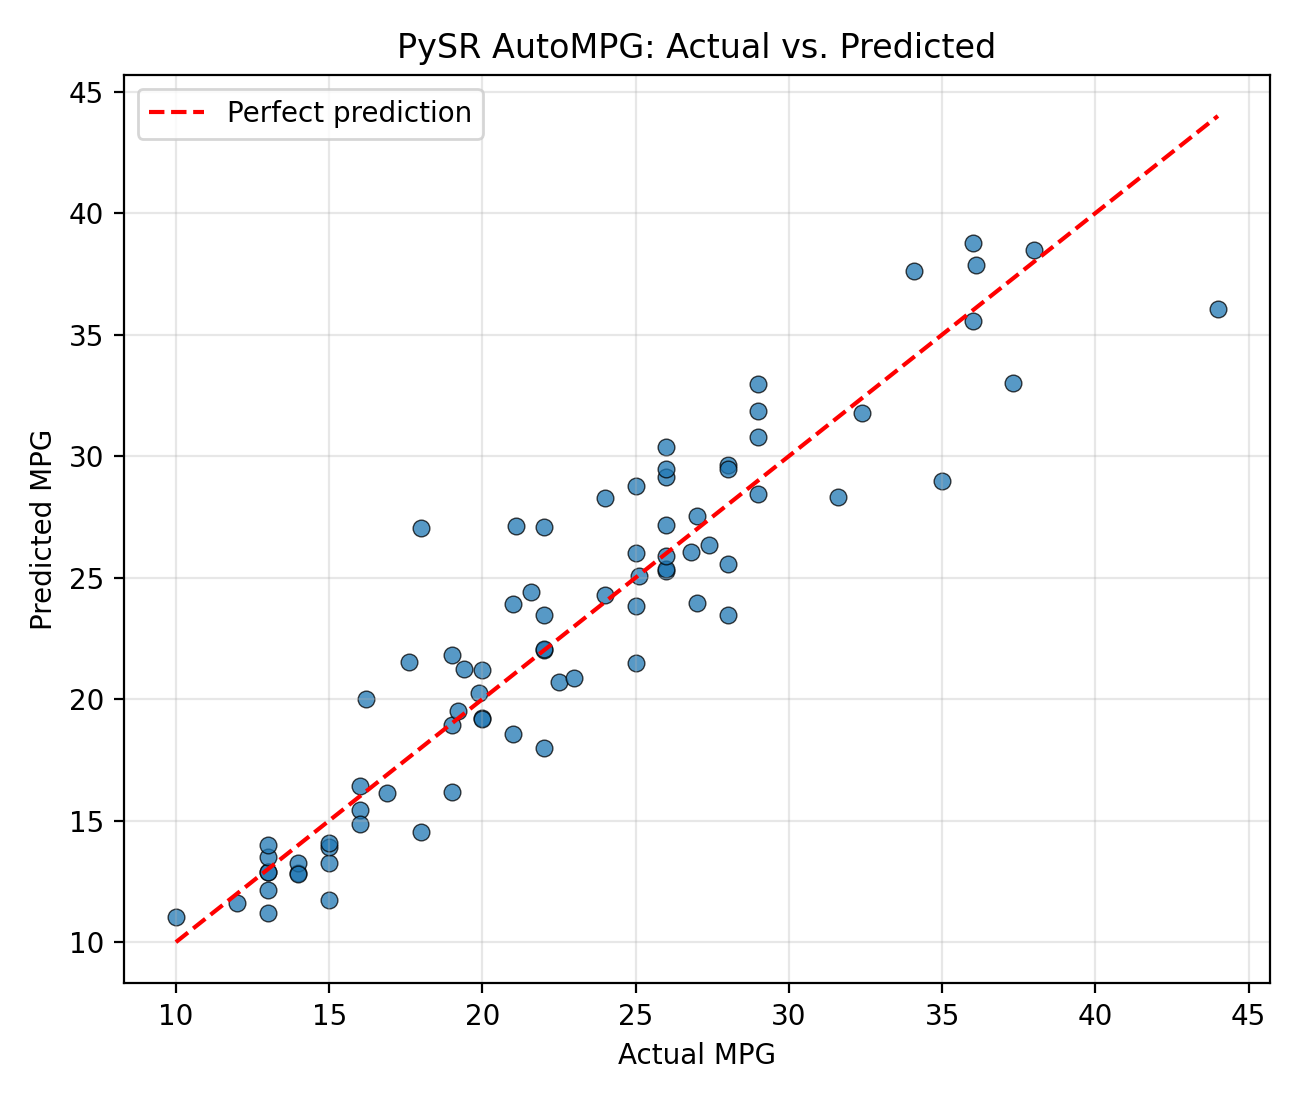
\includegraphics[width=0.60\textwidth]
    {Symbolic Regression Images/auto_mpg_pysr_actual_vs_predicted.png}
    \caption{Actual versus predicted MPG values for the PySR symbolic
    regression model. The dashed diagonal line represents perfect prediction.}
    \label{fig:pysr-auto}
\end{figure}

The predicted MPG values generally follow the perfect-prediction line,
indicating that the compact two-variable equation captures much of the
variation in MPG.

\subsubsection{Concrete}

The Concrete dataset contained 1030 observations and eight predictors:
cement, blast furnace slag, fly ash, water, superplasticizer, coarse
aggregate, fine aggregate, and age. The dataset was divided into 824
training observations and 206 testing observations.

PySR was run for 300 iterations with arithmetic operators and the nonlinear
operators \texttt{square}, \texttt{sqrt}, and \texttt{log}. The final
equation selected using the lowest training loss was

\begin{equation}
\begin{aligned}
\widehat{\mathrm{Strength}}
={}&-0.200393\,\mathrm{water}
+\sqrt{\mathrm{age}\,
\mathrm{superplasticizer}^{1/16}}
\\
&+1.201766
\sqrt{
\sqrt{\mathrm{fly\_ash}}
+\mathrm{slag}
-\frac{2.197127\,\mathrm{slag}}{\mathrm{age}}
}
\\
&+6.627109\log(\mathrm{age})
\\
&+1.201766
\log^2(\mathrm{cement})
\log^2\left(\log\left(\sqrt{\mathrm{cement}}\right)\right).
\end{aligned}
\end{equation}

The expression captures several nonlinear relationships. Water contributes
negatively, while age enters through both square-root and logarithmic terms.
The model also includes nonlinear contributions from slag, fly ash,
superplasticizer, and cement.

The held-out test performance was

\[
\mathrm{MSE}=42.3301,
\qquad
\mathrm{RMSE}=6.5062,
\]

\[
\mathrm{MAE}=5.3603,
\qquad
R^2=0.8357.
\]

\begin{figure}[H]
    \centering
    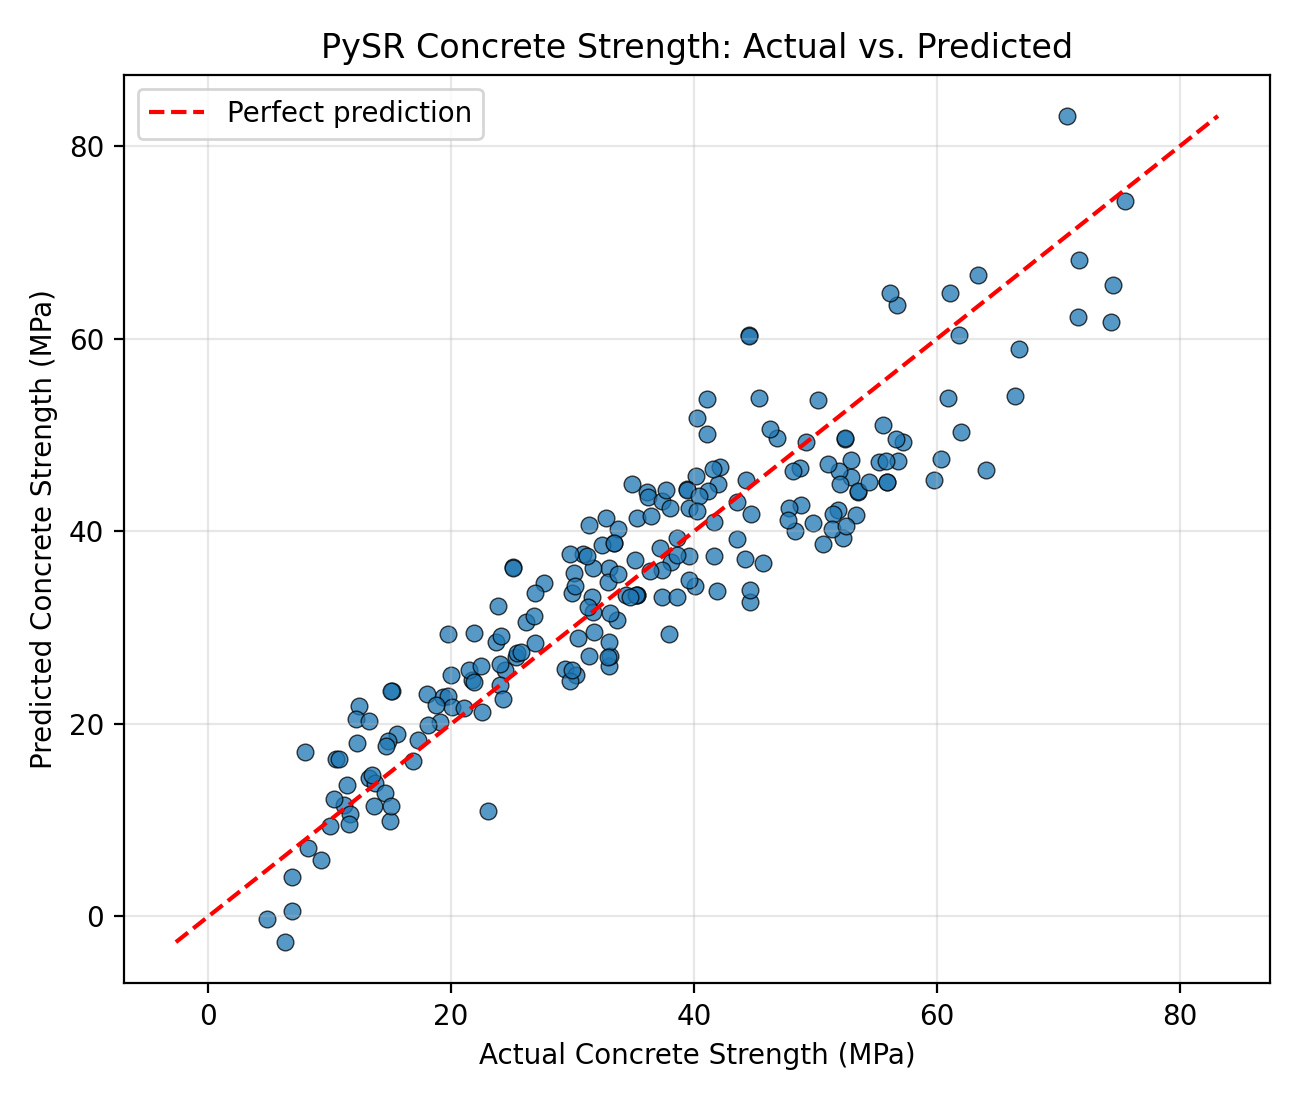
\includegraphics[width=0.60\textwidth]
    {Symbolic Regression Images/concrete_pysr_actual_vs_predicted.png}
    \caption{Actual versus predicted concrete compressive strength from
    the PySR symbolic regression model.}
    \label{fig:pysr-concrete}
\end{figure}

The model explains approximately 83.6\% of the variation in compressive
strength on the test data, indicating that the nonlinear expression captures
important relationships that are not represented by a simple linear model.

\subsubsection{Airfoil}

The Airfoil Self-Noise dataset contained 1503 observations with five
predictors: frequency, angle of attack, chord length, free-stream velocity,
and displacement thickness. The data were divided into 1202 training
observations and 301 testing observations.

PySR was run for 500 iterations using arithmetic operators together with
square, square-root, and logarithmic transformations. The selected symbolic
expression was

\begin{equation}
\begin{aligned}
\widehat{\mathrm{SPL}}
={}&
-\frac{
36.989017\,f
}{
f+
\left(
-195.3614\,d^2v+v
\right)^2
+128.70335+
\frac{2.3002949}{cd}
}
\\
&+136.76428
-\frac{
530.60527
}{
cf\log(195.3614d/c)
},
\end{aligned}
\end{equation}

where $f$ represents frequency, $v$ represents velocity, $c$ represents
chord length, and $d$ represents displacement thickness.

The model obtained the following test performance:

\[
\mathrm{MSE}=9.2244,
\qquad
\mathrm{RMSE}=3.0372,
\]

\[
\mathrm{MAE}=2.3529,
\qquad
R^2=0.8159.
\]

\begin{figure}[H]
    \centering
    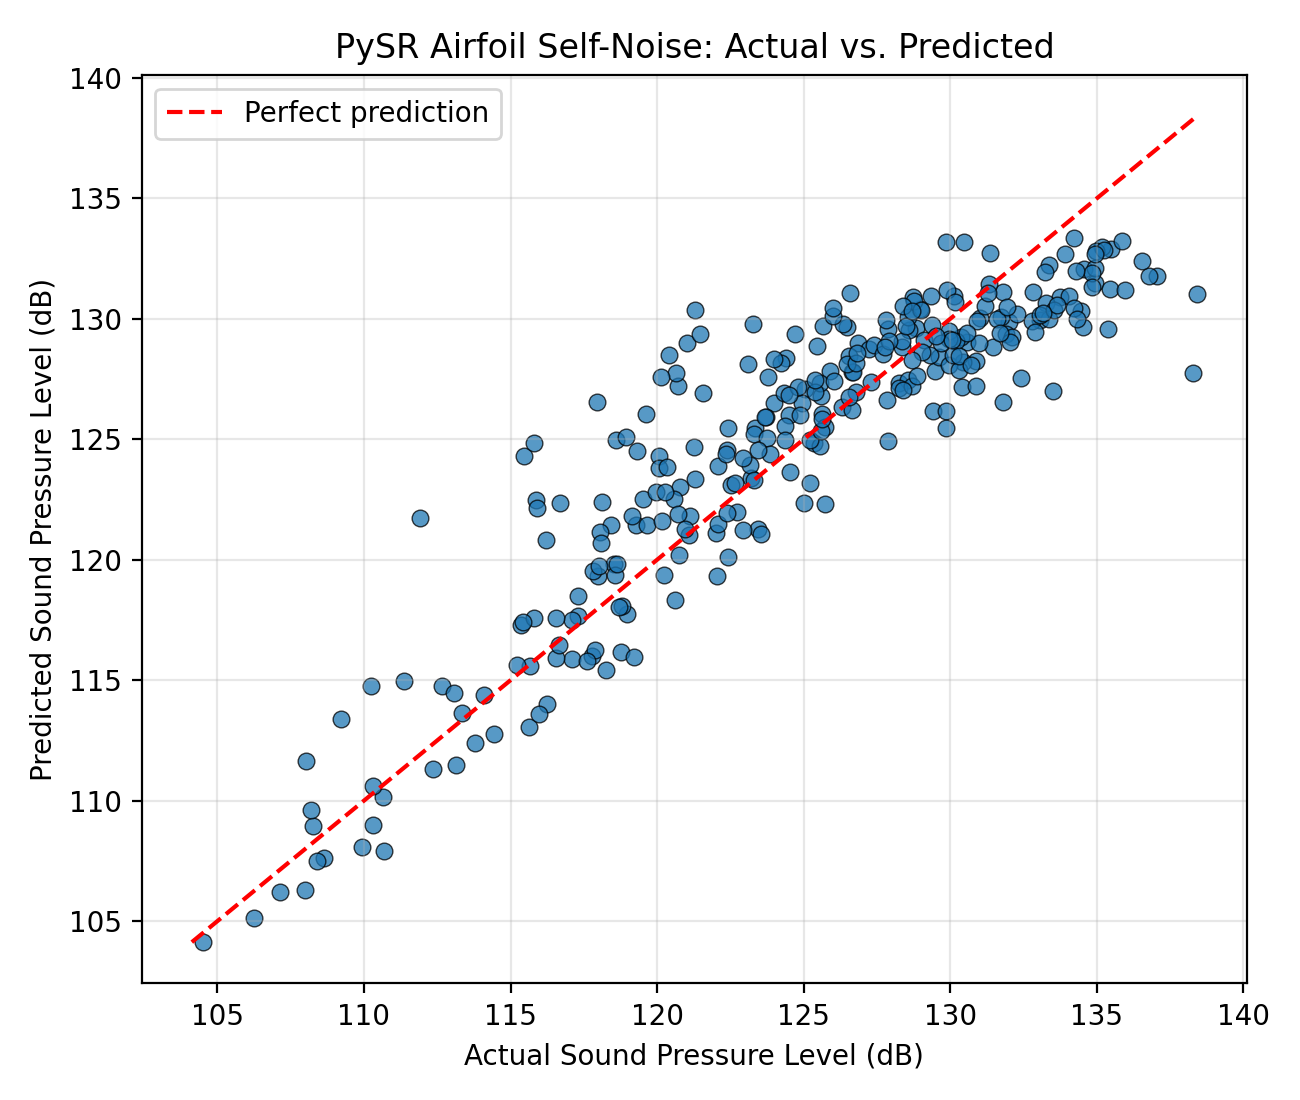
\includegraphics[width=0.60\textwidth]
    {Symbolic Regression Images/airfoil_pysr_actual_vs_predicted.png}
    \caption{Actual versus predicted sound pressure levels from the PySR
    symbolic regression model.}
    \label{fig:pysr-airfoil}
\end{figure}

The symbolic equation combines frequency, velocity, chord length, and
displacement thickness through nonlinear ratios and logarithmic terms. The
model explains approximately 81.6\% of the variation in sound pressure level
on the test set.

\subsection{Comparison of ScalaTion and PySR}

\begin{table}[H]
\centering\small
\caption{Symbolic regression on each tool's own test split. ScalaTion scores use the split-first procedure.}
\label{tab:symbolic-comparison}
\begin{tabular}{llrr}
\toprule
Dataset & Method & Test $R^2$ & RMSE \\
\midrule
Auto MPG & ScalaTion & 0.8650 & 2.7853 \\
 & PySR & 0.8519 & 2.7495 \\
Concrete & ScalaTion & 0.8237 & 6.8098 \\
 & PySR & 0.8357 & 6.5062 \\
Airfoil & ScalaTion & 0.7113 & 3.9985 \\
 & PySR & 0.8159 & 3.0372 \\
\bottomrule
\end{tabular}
\end{table}

Both methods provide explicit nonlinear expressions, but their search strategies and evaluation splits differ. ScalaTion builds a predefined nonlinear basis and selects terms from it, whereas PySR searches expression structures directly. ScalaTion uses Scala seed-42 shuffling and PySR uses scikit-learn's seed-42 split, so their test rows differ. These scores describe each experiment; they do not establish that one tool is better on a common test population.

Auto MPG has the largest ScalaTion test $R^2$ among its three datasets, and PySR gives a compact two-variable equation using weight and model year. For Concrete and Airfoil, PySR has lower reported test RMSE than the ScalaTion model on its own split. Within ScalaTion, all three selected symbolic models improve RMSE over linear regression evaluated on identical rows. The complete ScalaTion equations above expose every selected term, coefficient, and scaling constant; individual nonlinear coefficients require joint interpretation.

\end{document}
